%% Standard start of a latex document
\documentclass[letterpaper,12pt]{article}
%% Always use 12pt - it is much easier to read
%% Things written after '%' sign, are ignored by the latex editor - they are how to introduce comments into your .tex source
%% Anything mathematics related should be put in between '$' signs.

%% Set some names and numbers here so we can use them below
\newcommand{\name}{James Wu}

%%%%%%
%% There is a bit of stuff below which you should not have to change
%%%%%%

%% AMS mathematics packages - they contain many useful fonts and symbols.
\usepackage{amsmath, amsfonts, amssymb, bm}

%% The geometry package changes the margins to use more of the page, I suggest
%% using it because standard latex margins are chosen for articles and letters,
%% not homework.
\usepackage[paper=letterpaper,left=25mm,right=25mm,top=30mm,bottom=30mm]{geometry}
%% For details of how this package work, google the ``latex geometry documentation''.

%% Fancy headers and footers - make the document look nice
\usepackage{fancyhdr} %% for details on how this work, search-engine ``fancyhdr documentation''
\pagestyle{fancy}

\usepackage{graphicx}
\usepackage{adjustbox}

\setlength{\headheight}{15pt}

%% These put horizontal lines between the main text and header and footer.
\renewcommand{\headrulewidth}{0.4pt}
\renewcommand{\footrulewidth}{0.4pt}
%%%

%%%%%%
%% The above stuff is the same as the first template, but now we are starting to prove things, so we'd like to have a
%% good proof environment that gives us nice formatting and a little square at the end.
%% We'd also like a nice Result environment that prints that up nicely too.
%% Thankfully this exists in latex in the amsthm package
\usepackage{amsthm}
\newtheorem*{thm}{Theorem}
%% This creates a new theorem-like environment called "result", that will be titled "Result".
%% See below for examples of how to use this.
%%%%%%
\usepackage{enumitem}
%% This package allows us to make nice ordered lists with numbers, letters or roman numerals

\usepackage{titlesec}
\usepackage{hyperref}
\usepackage{tabularx}
\usepackage{ltablex}
\usepackage[justification=centering]{caption}
\usepackage{subcaption}
\usepackage{booktabs}
\newcolumntype{Y}{>{\centering\arraybackslash}X}

\usepackage{xcolor}
\definecolor{lblue}{HTML}{D8FFFF}
\definecolor{grellow}{HTML}{AEB55B}

\usepackage{listings}
\lstset{
    language=Python,
    frame=trbl,
    frameround=tttt,
    backgroundcolor=\color{lblue},
    rulecolor=\color{black},
    aboveskip=3mm,
    belowskip=3mm,
    showstringspaces=false,
    columns=flexible,
    basicstyle={\small\ttfamily},
    numbers=none,
    numberstyle=\tiny\color{gray},
    keywordstyle=\color{blue},
    commentstyle=\color{dkgreen},
    stringstyle=\color{grellow},
    breaklines=true,
    breakatwhitespace=true,
    tabsize=4,
    upquote=true,
}
\thicklines

\usepackage[hang,flushmargin]{footmisc}

\setlength{\parindent}{0em}
\setlength{\parskip}{0.5em}

\allowdisplaybreaks

\renewcommand{\arraystretch}{1.4}

\usepackage{empheq}

\newcommand*\wfbox[1]{\fbox{\hspace{0.4em}#1\hspace{0.4em}}}
\numberwithin{table}{section}
\numberwithin{figure}{section}
\numberwithin{equation}{section}

%% Useful commands
\renewcommand*{\qed}{\hfill\ensuremath{\square}}

\newcommand*{\uvec}[1]{\hat{\bm{#1}}}

\newcommand*{\deriv}[2]{\frac{d #1}{d #2}}
\newcommand*{\pderiv}[2]{\frac{\partial #1}{\partial #2}}
\newcommand*{\nderiv}[3]{\frac{d^{#3} #1}{d #2^{#3}}}
\newcommand*{\npderiv}[3]{\frac{\partial^{#3} #1}{\partial #2^{#3}}}
\newcommand*{\divg}[1]{\nabla \cdot \mathbf{#1}}
\newcommand*{\curl}[1]{\nabla \times \mathbf{#1}}

\newcommand*{\abs}[1]{\left| #1 \right|}
\newcommand*{\norm}[1]{\abs{\abs{\mathbf{#1}}}}

\newcommand*{\ev}[1]{\mathbb{E}\left[#1\right]}

\renewcommand*{\Re}[1]{\text{Re}\left(#1\right)}
\renewcommand*{\Im}[1]{\text{Im}\left(#1\right)}

\newcommand*{\qimg}[2]{\\ \begin{center}\includegraphics[scale=#1]{#2}\end{center}}

\newcommand*{\Arg}[1]{\text{Arg}\left(#1\right)}
\newcommand*{\Log}[1]{\text{Log}\left(#1\right)}
\newcommand*{\Tr}[1]{\text{Tr}\left(#1\right)}
\newcommand*{\Binom}[2]{\text{Binom}\left(#1, #2\right)}

\newcommand*{\ket}[1]{\left|#1\right>}
\newcommand*{\bra}[1]{\left<#1\right|}
\newcommand*{\braket}[2]{\left<#1\right|\left.\!#2\right>}
\newcommand*{\comm}[2]{\left[#1, #2\right]}

% Quick 2-vector and 2x2 matrix
\newcommand*{\qvec}[2]{\begin{pmatrix} #1 \\ #2 \end{pmatrix}}
\newcommand*{\qmat}[4]{\begin{pmatrix} #1 & #2 \\ #3 & #4 \end{pmatrix}}

% LaTeX
\newcommand{\fig}[2]{\includegraphics[width=#1\textwidth]{img/#2}}
\newcommand{\centerfig}[2]{\begin{center}\includegraphics[width=#1\textwidth]{img/#2}\end{center}}
\def\items#1{\begin{itemize}#1\end{itemize}}
\def\enum#1{\begin{enumerate}#1\end{enumerate}}
\newcommand{\ccaption}[1]{\caption{\textit{#1}}}

% References
\newcommand{\reffig}[1]{\textbf{Figure \ref{#1}}}
\newcommand{\reftab}[1]{\textbf{Table \ref{#1}}}
\newcommand{\refsec}[1]{\textbf{Section \ref{#1}}}

% Header
\lhead{}

%%

\begin{document}
\begin{flushleft}

    % TODO title page, etc.
    % TODO header, footer formatting

    \section{Preface}

    \subsection{Context}

    % Project context
    This four-month USRA project was undertaken with the supervision of Professor Wayne Nagata and Professor Priscilla Greenwood. Here we investigated the stochastic Morris-Lecar neuron, comparing different models and measuring statistics such as interspike interval (ISI) distributions and exit times.

    % About the report
    This report is a summary of the work the author has done, and serves as a companion to the codebase developed for this project. There are two types of readers this report targets: knowledgable researchers (such as Professor Priscilla and Professor Nagata) who can find results and code annotations handy in this report, and new students who would additionally benefit from the discussions of theory and resource recommendations.

    \subsection{Acknowledgements}

    % Thank supervisors
    I express my gratitude towards Professor Nagata and Professor Greenwood for introducing me to mathematical neuroscience, as well as engaging me more into nonlinear dynamics and stochastics. I have learned a lot from Professor Greenwood and Professor Nagata, and I thank them for supervising me.

    % Thank NSERC
    I also thank the Natural Sciences and Engineering Research Council of Canada for helping fund this project with a USRA.

    \subsection{Contact Me}
    I can be reached out to by email (as of the time of this writing) at \href{mailto:jwu277@gmail.com}{jwu277@gmail.com}.

    \pagebreak

    \section{Code Usage}

    The code developed for this project can be found (as of the time of this writing) at \url{https://github.com/jwu277/usra2021}. The software is written in Python 3.

    \subsection{Code Structure}

    % High-level description
    The project repoository is divided into three directories:
    \begin{enumerate}
        \item \texttt{neurons:} these files contain classes that are numerical implementations of various neuron models.
        \item \texttt{scripts:} these files contain runnable scripts that perform various simulations.
        \item \texttt{util:} these files contain various useful functions that files in the \texttt{neurons} and \texttt{scripts} directories may use.
    \end{enumerate}

    % Conventions to be aware of
    Functions and variables starting with an underscore (e.g. \texttt{\_a}) are intended to be used as private entities (i.e. only used within the file). Another thing is that each \texttt{neuron} file except for \texttt{neuron.mlr} has a corresponding \texttt{scripts} file with the same name that can be run for a quick simulation of the neuron. This mapping is not surjective, however. Now, some scripts will have a line similar to
    \begin{lstlisting}
        THREADS = 12
    \end{lstlisting}
    Feel free to change the number to the appropriate number of threads in your machine. Finally, scripts will sometimes have parameters such as \texttt{tmax}, \texttt{trials}, etc. As with most variables in the scripts, these can be changed to suit your needs.

    % Description of each file
    A description of the files in the repository is given in \reftab{tab:code-files}. Of course, the code files themselves contain more detailed annotations.
    
    \begin{center}
    
        \begin{tabularx}{\linewidth}{ | c | Y | X | }

            \hline
            File & Description & \multicolumn{1}{c|}{Notes} \\
            \hline\hline
            \texttt{neurons/bm.py} & Binary Markov (BM) neuron & \\
            \hline
            \texttt{neurons/izhikevich.py} & Izhikevich neuron & \\
            \hline
            \texttt{neurons/lif.py} & Linear integrate and fire neuron & \\
            \hline
            \texttt{neurons/ml.py} & Morris-Lecar neuron & \\
            \hline
            \texttt{neurons/mlj.py} & Jacobi Morris-Lecar neuron & Needs to be initialized with \texttt{init} before usage \\
            \hline
            \texttt{neurons/mll.py} & Linear Morris-Lecar neuron ($\tilde{\tilde{\mathbf{x}}}$) & Needs to be initialized with \texttt{init} before usage \\
            \hline
            \texttt{neurons/mlr.py} & Linear Modulus Morris-Lecar neuron & Not really used. Simulates the modulus of the linear Morris-Lecar neuron. \\
            \hline
            \texttt{neurons/modelb.py} & ``Model B'' neuron & Patched model still needs to be investigated further, so work can still be done here. \\
            \hline
            \texttt{scripts/bm.py} &  ISI distribution simulation for the binary Markov neuron & \\
            \hline
            \texttt{scripts/contour.py} & Generates FPE and ULC contours & \\
            \hline
            \texttt{scripts/det.py} & Compares deterministic trajectories of different neuron models & \\
            \hline
            \texttt{scripts/docheck.py} & Counts invalid oscillations in Model B2 & \\
            \hline
            \texttt{scripts/dtstab.py} & Compares different values of $dt$ and numerical methods (currently Euler and RK45) & $dt = 0.1$ suffices. Also, no appreciable difference was observed between the Euler and RK45 methods. \\
            \hline
            \texttt{scripts/elstats.py} & Generates statistical Poincare data for the FPE & \\
            \hline
            \texttt{scripts/isih.py} & ISI histogram generator for Morris-Lecar neuron & \\
            \hline
            \texttt{scripts/izhikevich.py} & ISI distribution simulation for the Izhikevich neuron with Poisson current & Not really used and might have inconsistent units \\
            \hline
            \texttt{scripts/lif.py} & ISI distribution simulation for the LIF neuron & \\
            \hline
            \texttt{scripts/longtin.py} & Simulation of Longtin's stochastic bistable system & Simulation does not reproduce Longtin's results \\
            \hline
            \texttt{scripts/ml.py} & Simulation of a single trajectory of the Morris-Lecar neuron & \\
            \hline
            \texttt{scripts/mlj.py} & Simulation of a single trajectory of the Jacobi Morris-Lecar neuron & \\
            \hline
            \texttt{scripts/mll.py} & Simulation of a single trajectory of the linear Morris-Lecar neuron & \\
            \hline
            \texttt{scripts/mlrtrials.py} & Simulates distribution of exit times for the \texttt{mlr} neuron & \\
            \hline
            \texttt{scripts/modelb.py} & Simulation of a single trajectory of the Model B neuron & \\
            \hline
            \texttt{scripts/pdist.py} & Simulates Poincare statistics for a fixed values of $\psi$ & \\
            \hline
            \texttt{scripts/phi\_noise.py} & Saves a run of Morris-Lecar neuron for certain values of$\phi$ and $N_K$ & Filename for save should be renamed as desired \\
            \hline
            \texttt{scripts/plotter.py} & Makes an animated plot of a phase portrait trajectory & Requires ImageMagick to be installed \\
            \hline
            \texttt{scripts/poincare.py} & Computes statistics for the $L$ Poincare section & \\
            \hline
            \texttt{util/current.py} & Generates $I(t)$ signal & \\
            \hline
            \texttt{util/dyn.py} & Used to find fixed point of a system & \\
            \hline
            \texttt{util/integrate.py} & Essentially a wrapper for \texttt{scipy.integrate.solve\_ivp
            } & \\
            \hline
            \texttt{util/isi.py} & Computes spike times and ISIs for neuron signals & Not useful for Morris-Lecar neuron. Used in BM, Izhikevich, and LIF neurons. \\
            \hline
            \texttt{util/ito.py} & Euler-Maruyama method implementation & \\
            \hline
            \texttt{util/ml.py} & Computes ISIs, orbit times, etc. for Morris-Lecar signals & \\
            \hline
            \texttt{util/plot.py} & Handy plotting functions & \\
            \hline

            \captionsetup{width=\linewidth}
            \ccaption{Descriptions of all the code files in the project repository. Note that much of the technical terminology is explained later in the report.}
            \label{tab:code-files}

        \end{tabularx}
    
    \end{center}

    \subsection{Running Scripts}
    First, a new user will likely need to run
    \begin{lstlisting}
        python -m pip install -r requirements.txt
    \end{lstlisting}
    in a terminal at the root of the repository. Note: \texttt{python} is taken to be the alias for Python 3. After that, the dependencies should be installed and scripts can now be run. To do so, execute
    \begin{lstlisting}
        python -m scripts.<scriptname>
    \end{lstlisting}
    in a terminal again at the root of the repository. Here \texttt{<scriptname>} is the name of the script file (excluding the \texttt{.py} suffix) to be run. For example, to run a simulation of ISIs for a binary Markov neuron, run
    \begin{lstlisting}
        python -m scripts.bm
    \end{lstlisting}
    As of the writing of this report, a plot should appear after a bit of computation time (exit the plot to terminate the program).

    \pagebreak

    \section{Morris-Lecar Neuron}
    
    \subsection{Circuit Model}

    % ML intro
    The Morris-Lecar description \cite{ml} models a neuron as having a membrane potential $v$, defined to be the difference in voltage between the inside and outside of the neuron cell. Current flows through potassium and calcium channels in the membrane, labelled as $I_K$ and $I_{Ca}$, respectively. There is also some current arising form other ions, which is collectively totalled as the leak current $I_L$. The combined potassium, calcium, and leak channels each have an effective conductance (or, taking reciprocals, resistance) and potential. Finally, the membrane has a capacitance $C$. \reffig{fig:ml-circuit} depicts a circuit for this model.

    % ML neuron circuit
    \begin{figure}[h]

        \centering
    
        \centerfig{0.6}{ml-circuit.jpg}

        \captionsetup{width=0.8\linewidth}
        \ccaption{Equivalent circuit of Morris-Lecar neuron model. Only $g_{Ca}$ and $g_K$ may vary with time--the other parameters in this diagram are constants. This diagram is copied from \cite{ml}.}
        \label{fig:ml-circuit}
    
    \end{figure}

    % ML circuit equation
    Consequently, the membrane potential obeys the following first order differential equation:
    \begin{equation}
        C\deriv{v}{t} = I - g_K (v - V_K) - g_{Ca} (v - V_{Ca}) - g_L (v - V_L)
        \label{eqn:ml-circuit}
    \end{equation}

    % ML conductances
    Nominally, the potassium and calcium conductances are non-constant. Rather, they obey the following equations:
    \begin{align}
        g_K &= \bar{g}_K w \\
        g_{Ca} &= \bar{g}_{Ca} m
    \end{align}
    where $\bar{g}_K, \bar{g}_{Ca}$ are constant.
    
    % ML voltage gating variables
    At constant $v$, the parameters $x = w, m$ are governed by first order differential equations of the following form:
    \begin{equation}
        \label{eqn:ml-voltage-gating}
        \deriv{x}{t} = \lambda_x(v) (x_\infty(v) - x)
    \end{equation}
    
    % ML voltage gating vars simplification
    However, the $m$ timescale is much shorter than the $w$ timescale, so that $m \approx m_\infty(v)$ in (\ref{eqn:ml-circuit}). Furthermore, to be consistent with \cite{snm}, we may re-arrange the $x = w$ version of (\ref{eqn:ml-voltage-gating}) to be of the following form:
    \begin{equation}
        \label{eqn:w-dyn}
        \deriv{w}{t} = \alpha(v)(1  - w) - \beta(v)w
    \end{equation}
    Finally, we have
    \begin{align}
        \label{eqn:alpha-def}
        \alpha(v) &= \frac{1}{2} \phi \cosh{\left(\frac{v - V_3}{2V_4}\right)}\left(1 + \tanh{\left(\frac{v - V_3}{V_4}\right)}\right) \\
        \label{eqn:beta-def}
        \beta(v) &= \frac{1}{2} \phi \cosh{\left(\frac{v - V_3}{2V_4}\right)}\left(1 - \tanh{\left(\frac{v - V_3}{V_4}\right)}\right) \\
        m_\infty(v) &= \frac{1}{2}\left(1 + \tanh{\left(\frac{v - V_1}{V_2}\right)}\right)
    \end{align}

    \subsection{Morris-Lecar Parameters}

    % Parameters table
    The parameters from \cite{snm} used in this project are given in \reftab{tab:ml-param}. Sometimes $I$ and/or $\phi$ are varied to assess the bifurcational behaviuor of the system.

    \begin{table}[h]

        \begin{subtable}{0.49\linewidth}

            \centering

            \begin{tabular}{ | c | c | c | }
                \hline
                Variable & Value & Units \\
                \hline\hline
                $C$ & 20 & $\mu F/cm^2$ \\
                \hline
                $g_L$ & 2.0 & $mS/cm^2$ \\
                \hline
                $\bar{g}_{Ca}$ & 4.4 & $mS/cm^2$ \\
                \hline
                $\bar{g}_K$ & 8 & $mS/cm^2$ \\
                \hline
                $V_L$ & -60 & $mV$ \\
                \hline
                $V_{Ca}$ & 120 & $mV$ \\
                \hline
                $V_K$ & -84 & $mV$ \\
                \hline
            \end{tabular}

        \end{subtable}
        \begin{subtable}{0.49\linewidth}

            \centering

            \begin{tabular}{ | c | c | c | }
                \hline
                Variable & Value & Units \\
                \hline\hline
                $V_1$ & -1.2 & $mV$ \\
                \hline
                $V_2$ & 18.0 & $mV$ \\
                \hline
                $V_3$ & 2.0 & $mV$ \\
                \hline
                $V_4$ & 30.0 & $mV$ \\
                \hline
                $\phi$ & 0.04 & $ms^{-1}$ \\
                \hline
                $I$ & 90 & $\mu A/cm^2$ \\
                \hline

            \end{tabular}

        \end{subtable}

        \captionsetup{width=0.85\linewidth}
        \ccaption{Values of parameters used in the Morris-Lecar model. These values are assumed for the remainder of the report unless specified otherwise.}
        \label{tab:ml-param}

    \end{table}

    \subsection{Helpful Resources}
    The books \cite{snm} and \cite{ermentrout} provide good introductions to the Morris-Lecar model.

    \pagebreak

    \section{Dynamics}

    \subsection{Bautin Bifurcation}

    % "Canonical" equation
    Consider a 2-dimensional dynamical system $(x(t), y(t)) \in \mathbb{R}^2$. We may equivalently define the complex variable $z = x + iy \in \mathbb{C}$. Alternatively, we may express this system in polar coordinates: $z = re^{i\varphi}$. Now, let us consider the system
    \begin{align}
        \deriv{z}{t} &= \lambda z\left(1 + k_1\abs{z}^2 + k_2\abs{z}^4 + O\left(\abs{z}^5\right)\right) \\
        \label{eqn:bautin-canon}
        &= \lambda z + c_1 z\abs{z}^2 + c_2 z\abs{z}^4 + O\left(\abs{z}^6\right)
    \end{align}
    Here $c_j = \lambda k_j$, and $\lambda, c_j \in \mathbb{C}$ for $j = 1, 2$. Let us rewrite $\lambda = \alpha + i\omega, c_j = l_j + im_j$, where $\alpha, \omega, l_j, m_j \in \mathbb{R}$. Then taking real and imaginary parts of (\ref{eqn:bautin-canon}) gets us
    \begin{align}
        \deriv{x}{t} &= (\alpha + l_1 r^2 + l_2 r^4)x - (\omega + m_1 r^2 + m_2 r^4)y \\
        \deriv{y}{t} &= (\omega + m_1 r^2 + m_2 r^4)x + (\alpha + l_1 r^2 + l_2 r^4)y
    \end{align}
    Here we dropped terms of order $O\left(\abs{z}^6\right)$ or higher. We do so by assuming that $l_2 < 0$ (and is thus nonzero). The parameter $l_2$, known as the \textit{second Lyapunov coefficient}, is indeed negative for the Morris-Lecar neuron (as we shall discuss later). Doing some calculus, the equations for $r$ and $\varphi$ become:
    \begin{align}
        \deriv{r}{t} &= r(\alpha + l_1 r^2 + l_2 r^4) \\
        \deriv{\varphi}{t} &= \omega + m_1 r^2 + m_2 r^4
    \end{align}

    % Fixed points + limit cycles
    We see that there is a fixed point at $r = 0$. Furthermore, there are circular limit cycles at $r^2$ satisfying the quadratic
    \begin{equation}
        \label{eqn:bautin-quad}
        f(r^2) = r^4 + \frac{l_1}{l_2} r^2 + \frac{\alpha}{l_2} = 0
    \end{equation}
    Since these limit cycles occur at $r > 0$, we have precisely one limit cycle for each $r^2$ root. The discriminant $\Delta$ of the quadratic (\ref{eqn:bautin-quad}) is
    \begin{equation}
        \Delta = \left(\frac{l_1}{l_2}\right)^2 - 4\frac{\alpha}{l_2} = \frac{1}{l_2^2} \left(l_1^2 - 4\alpha l_2\right)
    \end{equation}
    The sign of $\Delta$ is therefore just the sign of $l_1^2 - 4\alpha l_2$. Then a necessary condition for there to be limit cycles i.e. positive real roots for $r^2$ is:
    \begin{equation}
        \alpha \geq \frac{l_1^2}{4l_2}
    \end{equation}

    % Delta >= 0
    Now assuming that $\Delta \geq 0$ i.e. the roots for $r^2$ are all real, we use Vieta's formulas to note that the sum and product of the roots are $-\frac{l_1}{l_2}, \frac{\alpha}{l_2}$, repsectively.
    
    % alpha > 0
    For $\Delta \geq 0$, exactly one positive root exists precisely when $\alpha > 0 \therefore \frac{\alpha}{l_2} < 0$. But we immediately have $\alpha > 0 \geq \frac{l_1}{4l_2}$, satisfying the discriminant condition.

    % alpha = 0
    Now if $\alpha = 0$, then at least one root must coincide with $r = 0$. The other root is thus equal to $-\frac{l_1}{l_2}$ and is positive iff $l_1 > 0$.

    % alpha < 0
    Next, if $\alpha < 0$, both roots have the same sign. If $l_1 \leq 0$ then the sum of the roots is nonpositive, resulting in both roots being nonpositive. Thus there are no limit cycles for $\alpha < 0, l_1 \leq 0$. However, if $\alpha < 0$ and $l_1 > 0$, there are two positive roots for $r^2$ if $\alpha > \frac{l_1^2}{4l_2}$. If instead, $l_1 > 0$ and $\alpha = \frac{l_1^2}{4l_2} < 0$ then there is a repeated positive root and therefore one limit cycle.

    % Stability
    Finally, the stability of the limit cycles and $r = 0$ fixed point is determined by the sign of $f(r^2)$ in between these roots. Since $l_2 < 0$, the outermost limit cycle (or fixed point if none exists) attracts from $r = \infty$. Meanwhile, the stability of the fixed point is determined by the sign of $\alpha$ (or $l_1$ if $\alpha = 0$, or $l_2 < 0$ if $\alpha, l_1 = 0$). Finally, if there are two limit cycles, the inner one is unstable while the outer one is stable since $f(r^2)$ is a downwards parabola in $r^2$.

    % Bifurcation diagram
    Put all together, the bifurcation diagram is given in \reffig{fig:bautin}
    \begin{figure}[h]

        \centering
    
        \centerfig{0.65}{bautin.jpg}

        \captionsetup{width=0.8\linewidth}
        \ccaption{Bifurcation diagram of Bautin bifurcation. This figure was obtained from \cite{kuznetsov}. This diagram labels $\alpha$ and $l_1$ as $\beta_1$ and $\beta_2$, respectively.}
    
        \label{fig:bautin}
    
    \end{figure}

    % Hopf bifurcation
    The curve $H_- = \{\alpha = 0, l_1 < 0\}$, in \reffig{fig:bautin} is a \textit{Hopf bifurcation}. For a fixed $l_1 < 0$, varying $\alpha$ near zero affects the stability of the system; $\alpha < 0$ has a limit cycle whereas $\alpha > 0$ does not. Similarly, $H_+ = \{\alpha = 0, l_1 > 0\}$ is also a Hopf bifurcation. This time, a limit cycle is produced at the fixed point when varying $\alpha > 0$ to $\alpha < 0$. In general, the Hopf bifurcation is a local codim-1 bifurcation, where a limit cycle appears from/disappears into a fixed point.

    % SNLC bifurcation
    The curve $T = \{l_1 > 0, \alpha = \frac{l_1^2}{4l_2}\}$ is a \textit{saddle node of limit cycles (SNLC) bifurcation}. Here the two limit cycles in region 3 collapse into a single limit cycle on $T$. Varying a parameter more (e.g. decreasing $\alpha$ or $l_1$) will cause the semi-stable limit cycle to disappear. Like the Hopf bifurcation, the SNLC bifurcation is a local codim-1 bifurcation.

    % Bautin bifurcation
    Finally, a \textit{Bautin bifurcation} occurs near the point $\alpha, l_1 = 0$ in this model system. Since two parameters are varied in this bifurcation ($\alpha, l_1$), this is a local codim-2 bifurcation.

    \subsection{Morris-Lecar Dynamics}

    % Bautin bifurcation
    A Bautin bifurcation exists for the Morris-Lecar neuron in the parameters $(I, \phi)$ near $(I, \phi) = (90, 0.04)$. The bifurcation diagram is given in \reffig{fig:ml-bautin}.
    \begin{figure}[h]

        \centering
    
        \centerfig{0.8}{ml-bautin.jpg}

        \captionsetup{width=0.7\linewidth}
        \ccaption{Bautin bifurcation diagram, produced using \cite{matcont}. The red cross represents the origin of the Bautin bifurcation.}
    
        \label{fig:ml-bautin}
    
    \end{figure}
    We see that $(I, \phi) = (90, 0.04)$ corresponds to a system of type 3 in \reffig{fig:bautin}. The salient feature here is that there is a fixed point inside an unstable limit cycle inside a stable limit cycle. Corroborating this result, we keep $\phi = 0.04$ fixed and vary $I$ only. That gives us the bifurcation diagram in \reffig{fig:ml-bif1}.
    \begin{figure}[h]

        \centering
    
        \centerfig{0.8}{ml-bif1.jpg}

        \captionsetup{width=0.8\linewidth}
        \ccaption{Bifurcation diagram, produced using \cite{matcont}, with $\phi = 0.04$ fixed and $I$ varied. The value of $v$ at the fixed point, as well as extremal values of $v$ along the stable (SLC) and unstable (ULC) limit cycles are tracked.}
    
        \label{fig:ml-bif1}
    
    \end{figure}

    % Quiescent vs spiking oscillations
    In the $(v, w)$ phase plane, trajectories closing in on the fixed point represent \textit{quiescent} oscillations. In contrast, trajectories orbiting near the stable limit cycle exhibit \textit{spiking} oscillations. Since this system is bistable, these are the only types of oscillations that can arise. The switching between the quiescent and spiking states describe neuronal behaviour and is of interest to us. Example phase portraits and corresponding $v(t)$ signals of deterministic quiescent and spiking oscillations are given in \reffig{fig:q-plots} and \reffig{fig:s-plots}, respectively. Note that the phase portrait flows counterclockwise.

    \begin{figure}[!h]

        \centering
    
        % v(t)
        \begin{subfigure}{\textwidth}
            \centerfig{0.7}{qvt.jpg}
            \ccaption{$v(t)$ signal}
            \label{fig:q-plots-vt}
        \end{subfigure}

        % Phase portrait
        \begin{subfigure}{\textwidth}
            \centerfig{0.7}{qpp.jpg}
            \caption{Phase portrait}
            \label{fig:q-plots-pp}
        \end{subfigure}
    
        \captionsetup{width=0.9\linewidth}
        \ccaption{Quiescent trajectory with initial point $(-30.0, 0.15)$ and $t_{max} = 400$. As is the case for this report, voltage and time have units of $mV$ and $ms$, respectively.}
        \label{fig:q-plots}
    
    \end{figure}

    \begin{figure}[!h]

        \centering
    
        % v(t)
        \begin{subfigure}{\textwidth}
            \centerfig{0.7}{svt.jpg}
            \caption{$v(t)$ signal}
            \label{fig:s-plots-vt}
        \end{subfigure}

        % Phase portrait
        \begin{subfigure}{\textwidth}
            \centerfig{0.7}{spp.jpg}
            \caption{Phase portrait}
            \label{fig:s-plots-pp}
        \end{subfigure}
    
        \captionsetup{width=0.9\linewidth}
        \ccaption{Spiking trajectory with initial point $(-30.0, 0.1)$ and $t_{max} = 400$.}
        \label{fig:s-plots}
    
    \end{figure}

    % Running code
    These figures can be reproduced by running the \texttt{ml} script:
    \begin{lstlisting}
        python -m scripts.ml
    \end{lstlisting}
    To get a deterministic trajectory, set the \texttt{stochastic\_method} variable in the \texttt{scripts/ml.py} file to \texttt{None}:
    \begin{lstlisting}
        stochastic_method = None
    \end{lstlisting}
    For a quiescent trajectory, set the initial condition
    \begin{lstlisting}
        x0 = np.array([-30.0, 0.15])
    \end{lstlisting}
    and run the script. Meanwhile, for a spiking trajectory, set the initial condition
    \begin{lstlisting}
        x0 = np.array([-30.0, 0.1])
    \end{lstlisting}
    and run the script.

    \subsection{Scaling Results}

    % Attribute MatCont
    The results in this section were obtained with the use of \texttt{MATCONT} \cite{matcont}.

    % Im(eig) ~ sqrt(phi)
    Some potentially interesting scaling results in the Morris-Lecar neuron were obtained. First, along the $H_+$ curve in the Bautin bifurcation diagram, the fixed point has two imaginary eigenvalues that are conjugates of each other (since the real part goes to zero for Hopf bifurcations). It turns out that this imaginary part $\omega$ scales as $\sqrt{\phi}$:
    \begin{equation}
        \omega \sim \sqrt{\phi}
    \end{equation}

    This fit is compared to the numerical data in \reffig{fig:phi-im-scale}.
    \begin{figure}[h]

        \centering
 
        \centerfig{0.8}{phi-im-scale.jpg}
    
        \captionsetup{width=0.8\linewidth}
        \ccaption{Comparison of power law fit scaling and actual numerical data for $\omega(\phi)$ at small $\phi$. The fit obeys the equation $\omega = 0.4\sqrt{\phi}$.}
        \label{fig:phi-im-scale}
    
    \end{figure}

    This agrees with the theoretical result obtained in \cite{baer} (in that paper, the authors use $\varepsilon$ and $\lambda$ in place of $\phi$ and $I$, respectively).

    % Bifurcation curve fitting
    The scaling between $I$ and $\phi$ along the $H_+$ and SNLC curves for small $\phi$ was also investigated. Along the $H_+$ curve we have:
    \begin{equation}
        I - I_0 \sim \phi
    \end{equation}
    Along the SNLC curve we get:
    \begin{equation}
        I - I_0 \sim \phi^{4/3}
    \end{equation}
    Here $I_0 = 83.6$ is the value of $I$ in the $\phi \to 0^+$ limit (the $H_+$ and SNLC curves appear to approach the same point). These fits are compared to numerical data in \reffig{fig:bif-scale}.
    \begin{figure}[!h]

        \centering
 
        \centerfig{0.8}{bif-scale.jpg}
    
        \captionsetup{width=0.8\linewidth}
        \ccaption{Comparison of fit power law scaling and actual numerical data for $I(\phi)$ at small $\phi$ along the $H_+$ and SNLC bifurcation curves. The fits obey the relationships $I = 83.6 + 300 \: \phi$ and $I = 83.6 + 333.3 \: \phi^{4/3}$ along the $H_+$ and SNL curves, respectively.}
        \label{fig:bif-scale}
    
    \end{figure}

    \subsection{Helpful Resources}
    The book \cite{strogatz} provides an excellent introduction to bifurcation theory. A more advanced book on bifurcation theory is \cite{kuznetsov}. Meanwhile, the software \texttt{MATCONT} \cite{matcont}, which can be run through MATLAB, is really useful for numerical bifurcations. A helpful tutorial guide for \texttt{MATCONT} is \cite{matcont-tut}.

    \pagebreak

    \section{Stochastics}

    \subsection{It\^o Calculus}

    $X_t$ is a \textit{Wiener process} iff it is a continuous-time stochastic process satisfying the following conditions \cite{finbook}:
    \begin{enumerate}
        \item \textbf{Stationary increments:} If $s \leq t$, $X_t - X_s$ has the same distribution as $X_{t-s} - X_0$.
        \item \textbf{Independent increments:} If $s \leq t$, $X_t - X_s$ is independent of $X_r$ for all $r \leq s$.
        \item \textbf{Continuous paths:} $X_t$ is a continuous function of $t$.
    \end{enumerate}

    Here, a Wiener process is characterized by three paramters: the initial condition $X_0$, the drift $m$, and the variance parameter $\sigma^2$. For $s \leq t$, the increment $X_t - X_s$ is distributed as a Gaussian with mean $m(t - s)$ and variance $\sigma^2(t-s)$:
    \begin{equation}
        X_t - X_s \sim N\left(m(t - s), \sigma^2 (t - s)\right)
    \end{equation}
    The \textit{standard} Wiener process $B_t$ has $B_0 = 0$, $m = 0$, and $\sigma^2 = 1$. We may therefore write
    \begin{equation}
        dX_t = m dt + \sigma dB_t
    \end{equation}
    Note that $dB_t$ is distributed as
    \begin{equation}
        dB_t \sim \sqrt{dt}Z
    \end{equation}
    where $Z$ is a standard normal random variable. Now in general, if $f$ is a function of $X_t$, then we may write
    \begin{equation}
        df(X_t) = g(X_t) dt + h(X_t) dB_t
    \end{equation}
    for some functions $g(X_t), h(X_t)$ (It\^o's lemma gives a more precise result, but we will not utilize it for these purposes).

    The $n$-dimensional standard Wiener process $\mathbf{B_t}$ is simply a vector of $n$ independent standard Wiener processes. Then an $n$-dimensional dyanmical system $\mathbf{X}$ can be expressed in the form
    \begin{equation}
        \label{eqn:sde-general}
        d\mathbf{X} = \mathbf{g}(\mathbf{X}) dt + \mathbf{H}(\mathbf{X}) \mathbf{dB_t}
    \end{equation}
    Here $\mathbf{g}$ is a vector while $\mathbf{H}$ is a matrix.

    \subsection{Stochastic Morris-Lecar}

    % Stochastic model
    We can model the neuron as having $N_K$ potassium channels (in this project, we are typically on the order of $N_K \sim 1000$), each of which can be fully open or closed. The opening rate (i.e. probability rate of transition from the closed state to the open state) and closing rate for each channel would be $\alpha(v)$ and $\beta(v)$ from (\ref{eqn:w-dyn}), respectively. Then over a small time increment $dt$, the probability of a closed channel opening is $\alpha(v) dt$. Likewise, the probability of an open channel closing is $\beta(v) dt$.

    % Apply CLT
    Over a time increment of $dt$, we have
    \begin{equation}
        \label{eqn:w-stochastic-bare}
        dw = w(t + dt) - w(t) \sim \frac{\Binom{N_K (1 - w)}{\alpha dt} - \Binom{N_K w}{\beta dt}}{N_K}
    \end{equation}
    Note that $\Binom{n, p} = \sum_{j = 1}^n I_j$, where each $I_j$ is an independent indicator random variable with probability $p$. By the central limit theorem, when $n$ is large
    \begin{equation}
        \Binom{n}{p} \sim np + \sqrt{np(1-p)} Z
    \end{equation}
    where $Z$ is a standard normal random variable. Then (\ref{eqn:w-stochastic-bare}) becomes
    \small
    \begin{equation}
        dw \sim \frac{\left(N_K (1 - w) \alpha dt + \sqrt{N_K(1 - w) \alpha dt (1 - \alpha dt)}Z_1\right) - \left(N_K w \beta dt + \sqrt{N_K w \beta dt (1 - \beta dt)}Z_2\right)}{N_K}
    \end{equation}
    \normalsize
    Here $Z_1$ and $Z_2$ are independent normal random variables. This is because the closed and open channels are independent (as we assumed all the channels to be independent). Since $dt$ is small, $1 - \alpha dt \approx 1$. So
    \begin{equation}
        dw \sim \left(\alpha (1 - w) - \beta w\right) dt + \frac{1}{\sqrt{N_K}}\sqrt{\alpha (1 - w) + \beta w}\sqrt{dt}Z
    \end{equation}
    As a system of stochastic differential equations, we have
    \begin{align}
        \label{eqn:ml-stochastic}
        \qvec{v}{w}' &= \qvec{f(v, w)}{g(v, w)} dt + \qmat{0}{0}{0}{h(v, w)} \mathbf{dB_t} \\
        f(v, w) &= \frac{I - \bar{g}_K w (v - V_K) - \bar{g}_{Ca} m_\infty(v) (v - V_{Ca}) - g_L (v - V_L)}{C} \\
        g(v, w) &= \alpha(v) (1 - w) - \beta(v) w \\
        \label{eqn:ml-stochastic-end}
        h(v, w) &= \frac{1}{\sqrt{N_K}}\sqrt{\alpha(v) (1 - w) + \beta(v) w}
    \end{align}

    % Example stochastic trajectories
    Example phase portraits and corresponding $v(t)$ signals of stochastic quiescent and spiking oscillations are given in \reffig{fig:sq-plots} and \reffig{fig:ss-plots}. Note that the trajectory in \reffig{fig:sq-plots} transitions between quiescent and spiking states, as opposed to staying in the quiescent state like its deterministic counterpart. Such transitioning between quiescent and spiking states make the neuronal behaviour interesting and is worthy of closer investigation.

    \begin{figure}[!h]

        \centering
    
        % v(t)
        \begin{subfigure}{\textwidth}
            \centerfig{0.7}{sqvt.jpg}
            \caption{$v(t)$ signal}
            \label{fig:sq-plots-vt}
        \end{subfigure}

        % Phase portrait
        \begin{subfigure}{\textwidth}
            \centerfig{0.7}{sqpp.jpg}
            \caption{Phase portrait}
            \label{fig:sq-plots-pp}
        \end{subfigure}
    
        \captionsetup{width=0.85\linewidth}
        \ccaption{Stochastic trajectory with initial point $(-30.0, 0.15)$ and $t_{max} = 400$. Parts of the trajectory are quiescent while other parts are spiking.}
        \label{fig:sq-plots}
    
    \end{figure}

    \begin{figure}[!h]

        \centering
    
        % v(t)
        \begin{subfigure}{\textwidth}
            \centerfig{0.7}{ssvt.jpg}
            \caption{$v(t)$ signal}
            \label{fig:ss-plots-vt}
        \end{subfigure}

        % Phase portrait
        \begin{subfigure}{\textwidth}
            \centerfig{0.7}{sspp.jpg}
            \caption{Phase portrait}
            \label{fig:ss-plots-pp}
        \end{subfigure}
    
        \captionsetup{width=0.8\linewidth}
        \ccaption{Stochastic spiking trajectory with initial point $(-30.0, 0.1)$ and $t_{max} = 400$. Parts of this trajectory are quiescent.}
        \label{fig:ss-plots}
    
    \end{figure}

    \subsection{Euler-Maruyama Method}

    % General description
    The Euler-Maruyama method is a generalization of the Euler method to stochastic differential equations of the form (\ref{eqn:sde-general}). Here, a small finite time increment $dt$ is chosen. Then, starting from an initial condition $\mathbf{X}(0)$, we iteratively compute
    \begin{equation}
        \mathbf{X}(t + dt) = \mathbf{X}(t) + \mathbf{g}(\mathbf{X}) dt + \mathbf{H}(\mathbf{X}) \mathbf{Z} \sqrt{dt}
    \end{equation}
    Here $\mathbf{Z}$ is a randomly generated vector, where each entry is obtained from an independent unit normal distribution. The resulting path $\mathbf{X}(t)$ will be distributed approximately as the true distribution; thus, many trials of the Euler-Maruyama method can be used to obtain statistics for the process (e.g. ISIs, which will be discussed later).

    % ML-specific
    To ease computations, only the second entry of $\mathbf{Z}$ needs to be generated for the 2-dimensional stochastic Morris-Lecar model (since only $\mathbf{H_{22}}$ is nonzero). Furthermore, the random numbers can all be generated at the start rather than at every iteration.

    % Running code
    The Euler-Maruyama method is implemented in the project's software. One such script that utilizes this is \texttt{scripts/ml.py}. Here a stochastic trajectory of the Morris-Lecar neuron can be simulated using the Euler-Maruyama method. This can be done by first setting the appropriate stochastic method in the file:
    \begin{lstlisting}
        stochastic_method = 'euler'
    \end{lstlisting}
    Then the script can be run in a terminal:
    \begin{lstlisting}
        python -m scripts.ml
    \end{lstlisting}
    The plots in \reffig{fig:sq-plots} and \reffig{fig:ss-plots} can be reproduced (up to stochastic noise) by running this script with the Euler-Maruyama method.

    \subsection{Helpful Resources}
    The book \cite{finbook} provides a great introduction to stochastic calculus.

    \pagebreak

    \section{Interspike Intervals}

    One statistic of interest in this project is the ISI distribution. Intuitively, these intervals are the lengths of time between successive spikes in the membrane potential. Adding stochastics to the Morris-Lecar neuron results in a probabilistic distribution of intervals.

    \subsection{Defining Intervals}

    % How spike times are defined
    Defining interspike intervals boils down to defining spike times for a signal. Looking at the $v(t)$ signal in \reffig{fig:s-plots-vt}, we see that these ought to be the distinct local maxima in the $v(t)$ signal. However, not all $v(t)$ maxima qualify as spikes. For example, the quiescent signal in \reffig{fig:q-plots-vt} exhibits maxima, yet should not count as having any spikes. To complicate matters further, the noisy signals in \reffig{fig:sq-plots-vt} and \reffig{fig:ss-plots-vt} have both quiescent and spiking maxima. An easy way of differentiating these two maxima is to introduce a threshold (e.g. 20mV) that a maxima must exceed to constitute a spike.

    % Interspike intervals
    The ISIs in a signal can then be computed from the differences of these spike times. A given signal will typically have many spike times, giving rise to several ISIs. If we assume the stochastic Morris-Lecar neuron to be ergodic--which it ought to be at least approximately so, considering (granted, I have not proved this, or even gone much beyond \textit{considering} these assertions) that (a) the system can be expanded as an Ornstein–Uhlenbeck process near the fixed point and stable limit cycle, which should be ergodic, and (b) a finite transition probability exists between the two stable states--then running the system for a long time will give us the approximate ISI distribution.

    % Code
    Spike times and ISIs for a Morris-Lecar signal can be obtained using functions from the \texttt{util/ml.py} file. To reuse software components, the spike times are computed slightly differently than described in this section, however. \textit{Orbit times} (times at which an oscillation begins) are first computed, from which spiking times are determined. The orbit time calculation requires a \texttt{vdiff} parameter that represents at least how much maxima and minima of $v(t)$ should differ by. Meanwhile, the \texttt{sthresh} parameter is simply the spiking voltage threshold.

    \subsection{Results}

    % Introduce figures
    Numerically simulated ISI histograms for the stochastic Morris-Lecar neuron at various values of $N_K$ are given in \reffig{fig:isih}. Recall from (\ref{eqn:ml-stochastic-end}) that the noise amplitude is proportional to $N_K^{-1/2}$. The salient features of these histograms are the discrete peaks followed by the exponential tail.

    \begin{figure}[!h]

        \centering

        \begin{subfigure}{0.75\textwidth}
            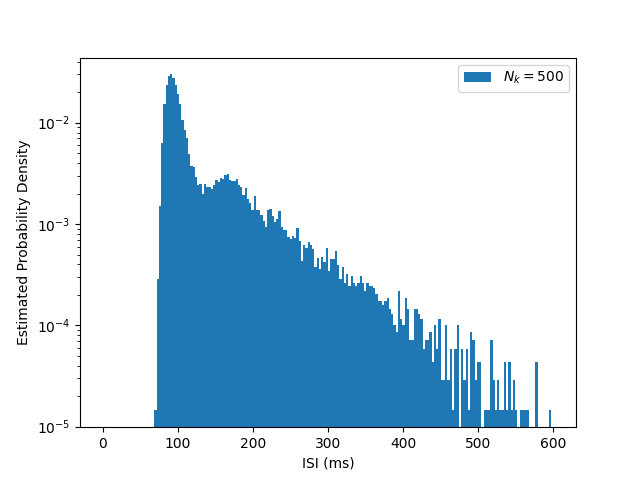
\includegraphics[width=\linewidth]{img/isih-nk500.jpg}
        \end{subfigure}
    
        \begin{subfigure}{0.75\textwidth}
            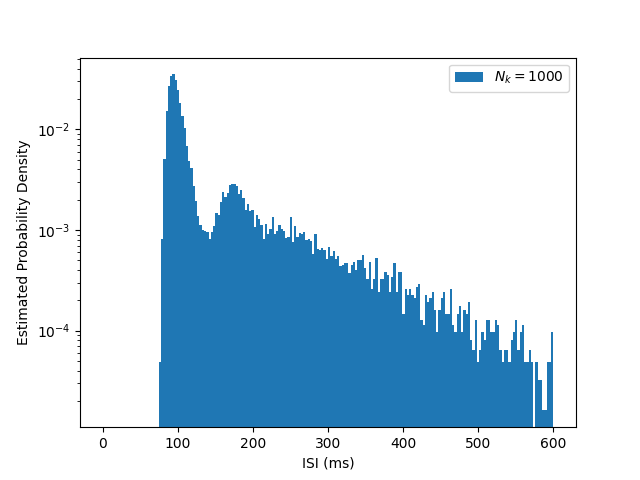
\includegraphics[width=\linewidth]{img/isih-nk1000.jpg}
        \end{subfigure}
        
        \ccaption{ISI histograms for various values of $N_K$. These histograms were produced by running 3200 trials of the Morris-Lecar neuron for 1000 ms each, with the initial point $(v, w) = (-40.0, 0.42)$.}

    \end{figure}
    \begin{figure}[!h]\ContinuedFloat

        \centering

        \begin{subfigure}{0.75\textwidth}
            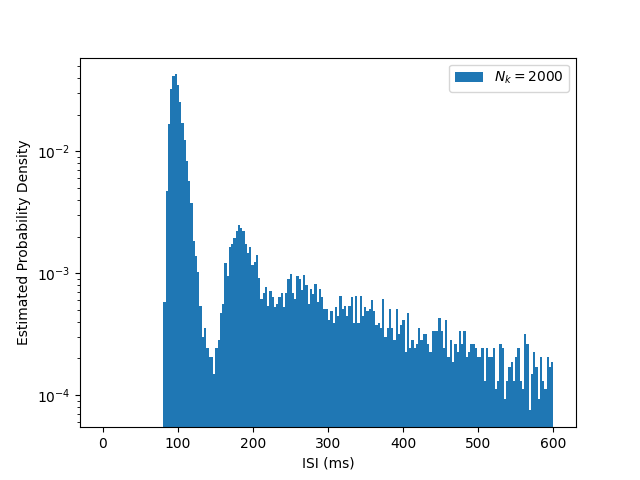
\includegraphics[width=\linewidth]{img/isih-nk2000.jpg}
        \end{subfigure}
    
        \begin{subfigure}{0.75\textwidth}
            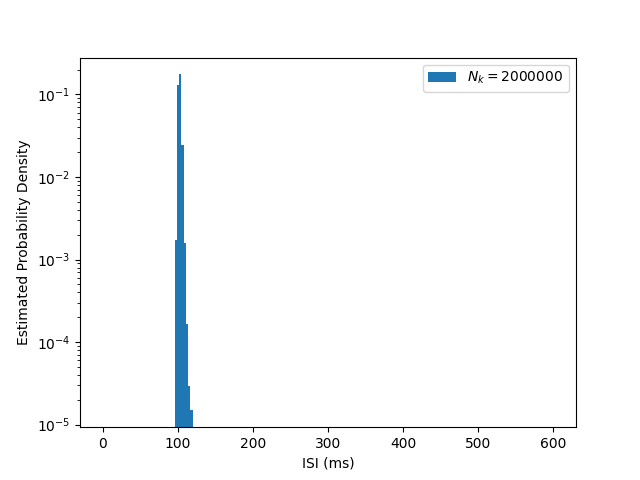
\includegraphics[width=\linewidth]{img/isih-nk2000000.jpg}
        \end{subfigure}

        \ccaption{ISI histograms for various values of $N_K$. These histograms were produced by running 3200 trials of the Morris-Lecar neuron for 1000ms each, with the initial point $(v, w) = (-40.0, 0.42)$. (cont.)}
        \label{fig:isih}

    \end{figure}

    % Explain features
    The discrete peaks and exponential tail can be explained as follows. Between every two consecutive spikes, there is one spiking oscillation and $n \geq 0$ quiescent oscillations. The total time $T$ between two such spikes is then
    \begin{equation}
        T = S + \sum_{i=1}^n Q_i
    \end{equation}
    where $S$ is the time duration of the spiking oscillation and $Q_i$ is the time duration of the $i$-th quiescent oscillation. As we might expect, $S$ and $Q_i$ are distributed unimodally with expectation values of approximately 100ms and 80ms, respectively. The standard deviations appear to be small compared to the EVs for these times.

    % Addition of RVs
    Thus the first discrete peak (ordering in terms of increasing ISI) corresponds to $n = 0$. Indeed, this peak is centred at around 100 ms, with the width being attributed to the deviation in $S$. Likewise, the second, third, etc. peaks correspond to $n = 1, 2$, etc. The centres of these peaks would be located at $100 + 80n$ milliseconds, with the width increasing with increasing $n$. This latter assertion arises from how standard deviation increases in quadrature as more independent RVs are added (we intuitively expect $S$ and $Q_i$ to be approximately independent--a claim we scrutinize more closely when we look at Poincare maps).

    % Exponentially decaying peak height
    We also expect the peak heights to decay exponentially with $n$. This can be seen from the following argument: if we assume quiescent oscillation to be approximately independent of each other, then each quiescent oscillation has a probability $p$ of transitioning to a spiking oscillation. Then $n \geq 1$ should follow a geometric distribution--hence the exponential decay in peak height.

    % Disappearance into tail
    Now, once $n$ becomes large enough, the successive peaks in the ISI histogram become so wide that they blend in with each other when superposed. The remaining feature of these blended peaks is therefore their heights (i.e. probability density) in the histogram. Per the previous discussion, this results in the exponential tail.

    % Code
    The numerically obtained ISI histograms agree with those found elsewhere, namely in \cite{rowat}. The results in this report can be reproduced using the \texttt{scripts.isih} script. Some parameters that can be changed in the script include \texttt{Nk}, \texttt{tmax}, and \texttt{epochs}. These correspond to $N_K$, the duration of a single trajectory, and the number of trajectories to simulate, respectively.

    \pagebreak

    \section{Poincare Maps}
    
    \subsection{Background}

    % Poincare sections
    A \textit{Poincare section} is a cross-sectional subset of a system's phase space that is transverse to oscillatory trajectories. For example, if we let $(v_{eq}, w_{eq})$ be the fixed point of the Morris-Lecar neuron, we can define the two Poincare sections $L, L'$ as:
    \begin{align}
        L &= \{(v, w) \: s.t. \: v = v_{eq}, w \leq w_{eq}\} \\
        L' &= \{(v, w) \: s.t. \: v = v_{eq}, w \geq w_{eq}\}
    \end{align}
    These subsets are depicted in \reffig{fig:pmap-def}.
    \begin{figure}[h]

        \centering
 
        \centerfig{0.9}{pmap-def.jpg}
    
        \captionsetup{width=0.75\linewidth}
        \ccaption{Plot of the Poincare sections in the $(v, w)$ phase plane. The fixed point and limit cycles are included for comparison.}
        \label{fig:pmap-def}
    
    \end{figure}

    % Poincare maps
    Indeed, trajectories such as those in \reffig{fig:q-plots} and \reffig{fig:s-plots} cross each of $L, L'$ once per oscillation. More formally, for a deterministic system, if we abbreviate $\mathbf{x}(t) = (v(t), w(t))$, then a time $t^*$ is a \textit{crossing time} through a Poincare section $S$ iff $\mathbf{x}(t) \in S$. So long as the trajectories are not tangent to the subset, there are only countably many crossing times. This is intuitively clear because trajectories must ``shoot through'' the section and cannot remain on it for more than an instant of time. We associate with every crossing time $t^*$ a \textit{crossing point} $\mathbf{x}(t^\ast) \in S$. We can thus define a function $P: S \to S$ for a Poincare section $S$, where $P(\mathbf{x}) = \mathbf{y}$ iff a trajectory starting at $\mathbf{x}$ has its next crossing point at $\mathbf{y}$ (the existence of $\mathbf{y}$ is guarenteed by how $S$ is transverse to oscillatory motion by definition; meanwhile, the uniqueness comes from the Well-Ordering Principle). The $P(\mathbf{x})$ function is known as a \textit{Poincare map}. We can similarly define the function $T(\mathbf{x}) : S \to \mathbf{R}$, where $T(\mathbf{x})$ is the next crossing time of a trajectory starting at $\mathbf{x}$. We shall call $T(\mathbf{x})$ the \textit{Poincare timer}.

    % Poincare section parameterization
    The $L$ and $L'$ sections are one-dimensional, so it helps to parametrize them by a single real parameter. Using the parameters $\psi, \psi' \geq 0$, we can parametrize $\psi \leftrightarrow (v_{eq}, w_{eq} - \psi)$ and $\psi' \leftrightarrow (v_{eq}, w_{eq} + \psi)$ for $L$ and $L'$, respectively. We then have the functions $P(\psi)$ and $T(\psi)$ (or $P(\psi')$ and $T(\psi')$) as the Poincare map and Poincare timer.

    % Examples
    As an example, the Poincare map for $L$ is plotted in \reffig{fig:pmap-det}.
    \begin{figure}[h]

        \centering
 
        \centerfig{0.8}{pmap-det.jpg}
    
        \captionsetup{width=0.75\linewidth}
        \ccaption{Deterministic Poincare map for the $L$ section.}
        \label{fig:pmap-det}
    
    \end{figure}
    Notice that there are three fixed points (i.e. $P(\psi) = \psi$) of the Poincare map. In order of increasing $\psi$, these correspond to the system's fixed point, unstable limit cycle, and stable limit cycle. Of course, fixed points of a deterministic Poincare map will always correspond to equilibria or limit cycles, and vice versa. The stability of the system's equilibria and limit cycles can then be inferred from the Poincare map. Here, we see that $P(\psi) < \psi$ for points between the fixed point and ULC. This implies that the fixed point is stable while the ULC is indeed unstable from the inside. This is because trajectories in this region move closer towards the fixed point after each oscillation. Similarly, the fact that $P(\psi) > \psi$ between the ULC and SLC further confirms that the ULC is unstable from the outside and that the SLC is stable from the inside. Finally, $P(\psi) < \psi$ outside the SLC shows that the SLC is indeed stable from the outside.

    % Stochastic Poincare map
    Finally, for a stochastic system, $P(\psi)$ and $T(\psi)$ are no longer real numbers but are instead random variables. The distributions of $P(\psi)$ and $T(\psi)$, and how they change with $\psi$ become of interest.

    \subsection{Numerical Implementation}
    \label{sec:pmap-numerical}

    % Description
    Crossing times for $L$ and $L'$ can be computed numerically from a given signal by first keeping track of $v_{eq}$ crossings for $v(t)$. In an e.g. Euler-Maruyama simulation, the signal will be an array of values $v[i]$, with $i$ being the index. The indices $i$ correspond to times $t_i$ i.e. $v[i] \approx v(t_i)$. Then since $v(t)$ crosses $L$ rightwards (recall that the trajectories flow counterclockwise in the phase plane), we check that $v[i] \leq v_{eq}$ and $v[i+1] \geq v_{eq}$. Finally, we check that the value of $w$ is correct: $w[i] \leq w_{eq}$. When these criteria are satisfied, $t_i$ is accepted as a crossing time. Likewise, $(v[i], w[i])$ is accepted as the associated crossing point. A similar case holds for $L'$ except $v[i] \geq v_{eq}$, $v[i+1] \leq v_{eq}$, and $w[i] \geq w_{eq}$.

    % Code
    The \texttt{scripts.poincare} script uses this logic to compute $P(\psi)$ and $T(\psi)$ distributions, as well as how frequently a given oscillation spikes for a certain $\psi$.

    \subsection{Results}

    % Summary of P(psi), T(psi), spiking probability
    For noise at the $N_K = 2000$ level (recall that noise amplitude is proportional to $N_K^{-1/2}$), the distinct sigmoid shape of the Poincare map in \reffig{fig:pmap-det} (we consider $\ev{P(\psi)}$ for the stochastic system) disappears. Of course, there are levels of noise that are weak enough to retain the sigmoidal shape of $\ev{P(\psi)}$ while still having an appreciable variance in $P(\psi)$. This latter quality allows for transitions between spiking and quiescent states, and gives rise to a distribution of ISIs. Plots of $\ev{P(\psi)}$, $\ev{T(\psi)}$, and spiking probabilities versus $\psi$ for $N_K = 2000, 2 \times 10^6$ are given in \reffig{fig:poincare}.

    \begin{figure}[!h]

        \centering

        \begin{subfigure}{0.72\textwidth}
            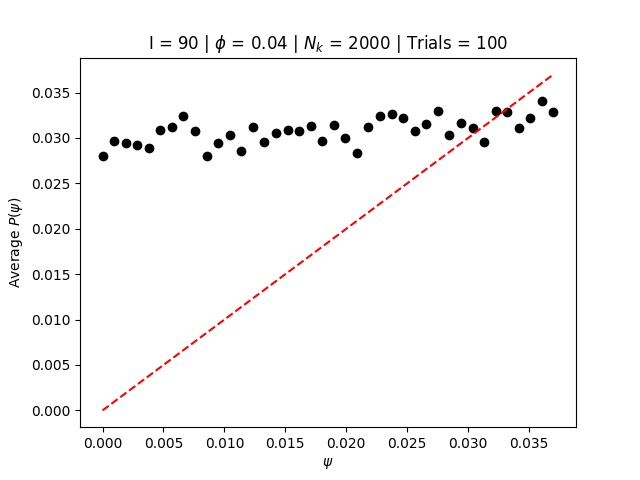
\includegraphics[width=\linewidth]{img/pmap-nk2000.jpg}
            \caption{$\ev{P(\psi)}$ versus $\psi$ for $N_K = 2000$}
        \end{subfigure}
    
        \begin{subfigure}{0.72\textwidth}
            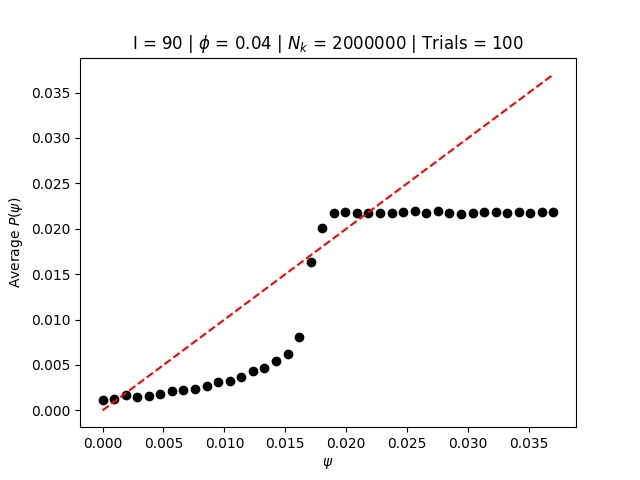
\includegraphics[width=\linewidth]{img/pmap-nk2000000.jpg}
            \caption{$\ev{P(\psi)}$ versus $\psi$ for $N_K = 2000000$}
        \end{subfigure}
        
        \captionsetup{width=0.8\linewidth}
        \ccaption{Plots of various Poincare statistics. Each of the 100 trials constituted running a single oscillation for every value of $\psi$.}

    \end{figure}
    \begin{figure}[!h]\ContinuedFloat

        \centering

        \begin{subfigure}{0.72\textwidth}
            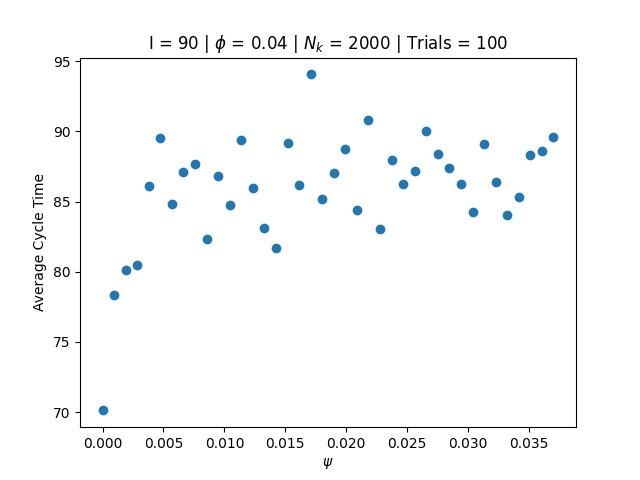
\includegraphics[width=\linewidth]{img/pt-nk2000.jpg}
            \caption{$\ev{T(\psi)}$ versus $\psi$ for $N_K = 2000$}
        \end{subfigure}
    
        \begin{subfigure}{0.72\textwidth}
            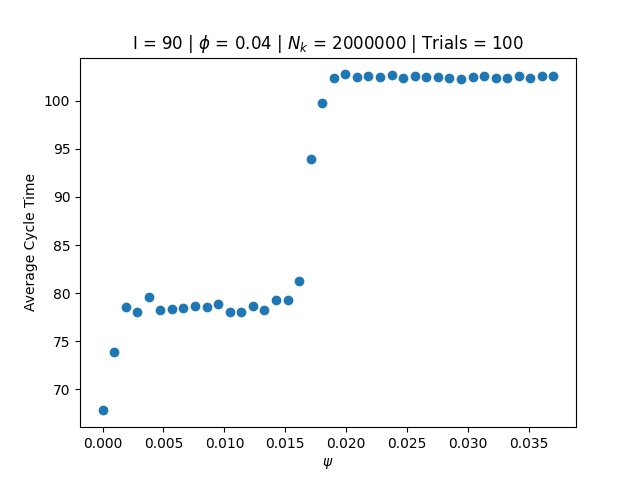
\includegraphics[width=\linewidth]{img/pt-nk2000000.jpg}
            \caption{$\ev{T(\psi)}$ versus $\psi$ for $N_K = 2000000$}
        \end{subfigure}

        \captionsetup{width=0.8\linewidth}
        \ccaption{Plots of various Poincare statistics. Each of the 100 trials constituted running a single oscillation for every value of $\psi$. (cont.)}

    \end{figure}
    \begin{figure}[!h]\ContinuedFloat

        \centering

        \begin{subfigure}{0.72\textwidth}
            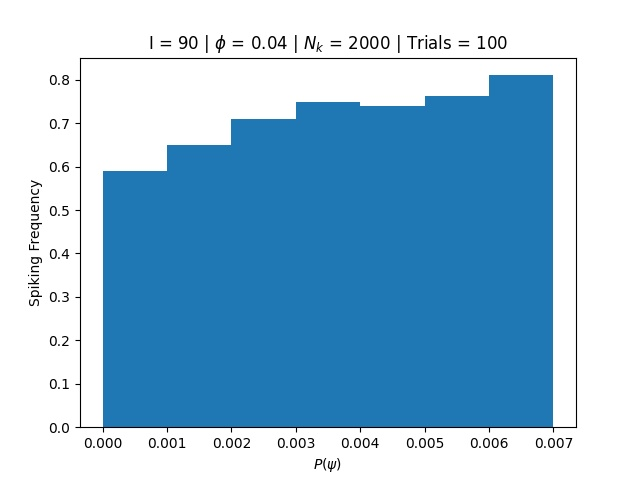
\includegraphics[width=\linewidth]{img/pspike-nk2000.jpg}
            \caption{Spiking frequency versus $\psi$ for $N_K = 2000$}
        \end{subfigure}
    
        \begin{subfigure}{0.72\textwidth}
            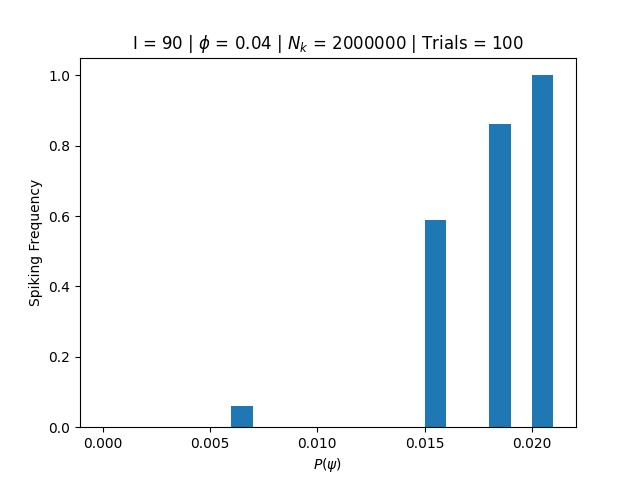
\includegraphics[width=\linewidth]{img/pspike-nk2000000.jpg}
            \caption{Spiking frequency versus $\psi$ for $N_K = 2000000$}
        \end{subfigure}

        \captionsetup{width=0.8\linewidth}
        \ccaption{Plots of various Poincare statistics. Each of the 100 trials constituted running a single oscillation for every value of $\psi$. (cont.)}
        \label{fig:poincare}

    \end{figure}

    % pdist
    For weak noise (e.g. $N_K = 2 \times 10^6$), the $P(\psi)$ distributions is bimodal when $\psi$ is near the ULC i.e. $\psi \approx 0.017$. If $\psi$ is much more or less than this, the distribution becomes seemingly unimodal. A few of these simulated distributions are given in \reffig{fig:pdist}.
    \begin{figure}[!h]

        \centering

        \begin{subfigure}{0.75\textwidth}
            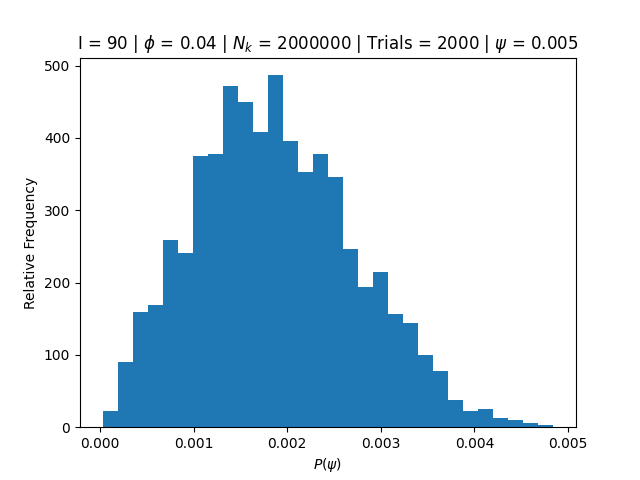
\includegraphics[width=\linewidth]{img/pdist-psi0005.jpg}
            \caption{$\psi = 0.005$}
            \label{fig:pdist-psi0005}
        \end{subfigure}

        \begin{subfigure}{0.75\textwidth}
            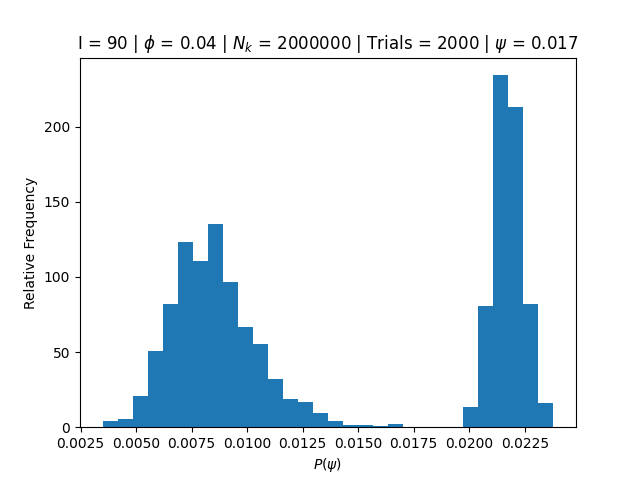
\includegraphics[width=\linewidth]{img/pdist-psi0017.jpg}
            \caption{$\psi = 0.017$}
            \label{fig:pdist-psi0017}
        \end{subfigure}

        \captionsetup{width=\linewidth}
        \ccaption{Simulation of the distribution of $P(\psi)$ for various values of $\psi$.}

    \end{figure}
    \begin{figure}[!h]\ContinuedFloat

        \centering
    
        \begin{subfigure}{0.75\textwidth}
            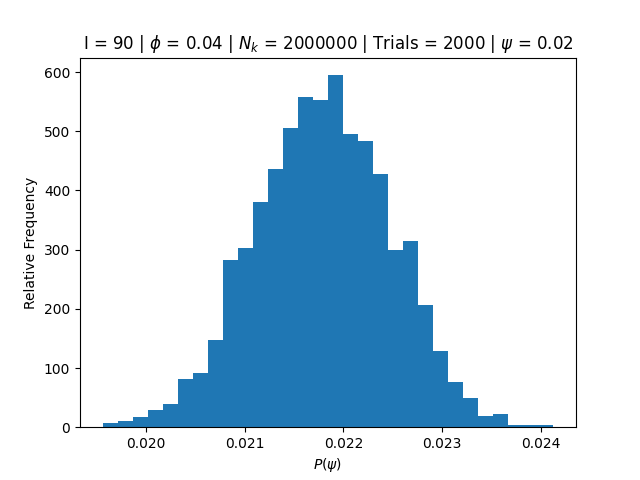
\includegraphics[width=\linewidth]{img/pdist-psi002.jpg}
            \caption{$\psi = 0.02$}
            \label{fig:pdist-psi002}
        \end{subfigure}

        \captionsetup{width=\linewidth}
        \ccaption{Simulation of the distribution of $P(\psi)$ for various values of $\psi$. (cont.)}
        \label{fig:pdist}

    \end{figure}

    % Explain pdist
    One explanation of the unimodal/bimodal distributions is that the modes correspond to the stable states of the system i.e. the fixed point and SLC. So inside the ULC, the system will be attracted to the fixed point and therefore exhibit the distribution associated with the fixed point (as in \reffig{fig:pdist-psi0005}). Now, outside the ULC, the system is attracted to the SLC and thus produces the corresponding mode (as in \reffig{fig:pdist-psi002}). However, near the ULC, the stochastic noise can push the trajectory across to either side of the ULC. This results in a superposition of the fixed point and SLC modes in the histogram (as in \reffig{fig:pdist-psi0017}).

    % Explain centering of modes
    The mode associated with the SLC is indeed maximal at approximately the value of $\psi$ corresponding to the SLC (i.e. the intersection of the SLC and $L$). However, the mode associated with the fixed point is not maximal at $\psi = 0$, where the fixed point is located. One reason this discrepancy arises is that the SLC attraction is strong in the sense that deterministic trajectories typically converge near it within one oscillation. In contrast, trajectories will spiral towards the fixed point (at the speed of exponentially decay) as seen in \reffig{fig:q-plots-pp}. So if we naively assume the modes to be maximal at the deterministic $P(\psi)$, we would expect the SLC mode to exist as such and the fixed point mode to be offset from $\psi = 0$. Another reason for the offset is the one-sidedness of $L$ i.e. that $\psi$ is nonnegative. To illustrate, if a deterministic were to reach a small neighbourhood of the fixed point (for concreteness we make the neighbourhood diameter much smaller than the noise amplitude multiplied by the square root of the time scale i.e. the oscillation period ~ 80 ms), Brownian motion in \textit{any} direction will cause a deviation from the fixed point. If the system is perturbed in direction of decreasing $w$, $P(\psi)$ would increase as usual. However, if the system is instead disturbed in the direction of increasing $w$, the trajectory will be above the fixed point and effectively become a trajectory that is halfway through an oscillation; the phase portrait will then circle around and hit $L$ at a location below the fixed point.

    % Code: poincare
    The script used to generate the various Poincare statistics in \reffig{fig:poincare} can be found in \texttt{scripts.poincare}. Variables of interest to change are \texttt{Nk}, \texttt{psi\_range} (which defines the values of $\psi$ to be probed) and \texttt{trials} (the number of trials to perform). 
    
    % Code: pdist
    Meanwhile, the script used to generate the distributions of $P(\psi)$ for specific values of $\psi$ is contained in \texttt{scripts.pdist}. This script additionally generates histograms for $T(\psi)$ and spiking frequency for fixed $\psi$. Some variables to change here include \texttt{Nk}, \texttt{psi}, and \texttt{trials}. The reader is encouraged to run these scripts for themselves should they wish to collect more data (e.g. with different parameters) or reproduce these results.

    \pagebreak

    \section{Alternative Dynamics}

    \subsection{Jacobi Dynamics}

    % Motivation
    Physically, $w$ should be bounded in $[0, 1]$. However, the equations described in (\ref{eqn:ml-stochastic})-(\ref{eqn:ml-stochastic-end}) imply a finite (albeit small) possibility of $w$ being outside of $[0, 1]$. \textit{In practice}, this issue never really manifests. For theoretical satisfaction, however, we may instead use--for a fixed $v$--a bounded diffusion process for $w$.

    % Jacobi diffusion
    Following \cite{dg}, we choose the simplest diffusion process that mimics the system. Arguably, we wish to preserve the dynamic part $g(v, w)$ while having as simple of a variance coefficient $h(v, w)^2$ as possible. The preservation of $g(v, w)$ can be vouched for as it, loosely speaking, determines the ``average'' behaviour of the system, as well as defining the $N_K \to 0$ limit behaviour. Seeing that $g(v, w)$ is linear in $w$, we consider Pearson diffusions, where $h(v, w)^2$ is a polynomial of degree at most two. It turns out that the Jacobi diffusion is the only Pearson diffusion bounded in a finite interval. This renders a Jacobi diffusion as the ``simplest'' bounded diffusion process appropriate for the stochastic Morris-Lecar system.

    % Ergodicity
    We follow the discussion \cite{dg} on the Jacobi diffusion here. The Jacobi diffusion bounded on $(0, 1)$ has the form (for fixed $v$)
    \begin{equation}
        \label{eqn:w-jacobi-base}
        dw = -\theta (w - \mu) dt + \gamma\sqrt{2\theta w (1 - w)} dB_t
    \end{equation}
    Equating the dynamic part gets us
    \begin{equation}
        \theta = \alpha + \beta, \quad \mu = \frac{\alpha}{\alpha + \beta}
    \end{equation}
    Note that we necessarily have $\alpha(v), \beta(v) \geq 0$ as can be seen from (\ref{eqn:alpha-def})-(\ref{eqn:beta-def}). The Jacobi diffusion is \textit{ergodic} for
    \begin{equation}
        \label{eqn:jacobi-ergodic-condition}
        \gamma^2 \leq \mu, 1 - \mu
    \end{equation}
    To retain this property, we can rewrite $\gamma = \sigma^* \delta(v)$, where $\sigma^*$ is a constant that can be fit (to e.g. match $h(v, w)$ at the fixed point) and $\delta(v)$ is a simple function of $v$. Of course, such a choice of $\sigma^*, \delta(v)$ is not unique since we can rewrite $\sigma^* \mapsto x\sigma^*$, $\delta(v) \mapsto \frac{\delta(v)}{x}$ for any nonzero $x$. We therefore assert the condition that $\sigma^* \in [0, 1]$ and that (\ref{eqn:jacobi-ergodic-condition}) holds for all $\sigma^*$ in that range. When fitting $\sigma^*$, the ergodicity requirement becomes verifying that $\sigma^* \in [0, 1]$.

    % Jacobi parameters
    $\gamma^2$ is largest when $\sigma^* = 1$, so our task becomes assuring that $\delta(v)^2 \leq \mu, 1 - \mu$ i.e.
    \begin{equation}
        \delta(v)^2 \leq \frac{\alpha(v)}{\alpha(v) + \beta(v)}, \frac{\beta(v)}{\alpha(v) + \beta(v)}
    \end{equation}
    Naively, we could define
    \begin{equation}
        \delta(v) = \sqrt{\min{\left(\frac{\alpha(v)}{\alpha(v) + \beta(v)}, \frac{\beta(v)}{\alpha(v) + \beta(v)}\right)}}
    \end{equation}
    However, the piecewise definition comes at the cost of differentiability. To make $\delta(v)$ analytically ``well-behaved'', we instead define $\delta(v)^2$ to be the harmonic sum of $\mu, 1 - \mu$ (as is done for e.g. parallel resistors):
    \begin{equation}
        \delta(v)^2 = \frac{\mu(1 - \mu)}{\mu + (1 - \mu)} = \frac{\alpha\beta}{\alpha + \beta}
    \end{equation}
    Thus
    \begin{equation}
        \gamma = \sigma^* \sqrt{\frac{\alpha\beta}{\alpha + \beta}}
    \end{equation}
    Equation (\ref{eqn:w-jacobi-base}) now becomes
    \begin{equation}
        \label{eqn:w-jacobi}
        dw = (\alpha(v) (1 - w) - \beta(v) w) dt + \sigma^* \sqrt{2\frac{\alpha(v)\beta(v)}{\alpha(v) + \beta(v)} w(1-w)} dB_t
    \end{equation}

    % sigma* fitting
    The fixed point of the system occurs at approximately $(v_{eq}, w_{eq}) = (-26.6, 0.129)$. Plugging this into (\ref{eqn:ml-stochastic-end}) and the coefficient in front of $dB_t$ in (\ref{eqn:w-jacobi}) gives
    \begin{equation}
        \label{eqn:h-eq}
        h(v_{eq}, w_{eq}) = \frac{0.1003}{\sqrt{N_K}} = 0.03365\sigma^*
    \end{equation}
    That gives us
    \begin{equation}
        \sigma^* = \frac{2.98}{\sqrt{N_K}}
    \end{equation}
    Since $N_K$ is on the order of $1000$, and certainly larger than $9$, we see that typical fits of $\sigma^*$ are indeed ergodic.

    \subsection{Linearized Dynamics}
    
    % Linear equation
    Near the fixed point, we can expand (\ref{eqn:ml-stochastic}) as a linear model as in \cite{dg}. Since the deterministic part is zero to zeroth order, we expand it to first order. In contrast, the stochastic part $h(v, w)$ is nonzero to zeroth order, so we need only expand that to zeroth order. That gets us
    \begin{equation}
        \label{eqn:mll}
        \qvec{v}{w}' \approx \mathbf{M} \qvec{v}{w} dt + \qvec{0}{\frac{0.1003}{\sqrt{N_K}} dB_t}
    \end{equation}
    Here we used the value of (\ref{eqn:h-eq}) for the stochastic part. Meanwhile, $\mathbf{M}$ is the Jacobian matrix of the dynamic part in (\ref{eqn:ml-stochastic}):
    \begin{equation}
        \mathbf{M} = D\qvec{f(v, w)}{g(v, w)}
    \end{equation}

    % X~ transformation
    The linear approximation is valid in a small region near the fixed point. Of course, this region is necessarily within the unstable limit cycle. Numerical experiemnts can provide more clarity into the size of this region. Such a region would be elliptical, however. This is because the coordinates $v, w$ are not symmetrical in the sense that $\mathbf{M}$ does not stretch and shear them uniformly. To remove this complication and simplify the equation, we can define the matrix
    \begin{equation}
        \mathbf{Q} = \qmat{\omega}{m_{11} + \lambda}{0}{m_{21}}
    \end{equation}
    Then we define
    \begin{align}
        \mathbf{A} &= \mathbf{Q}^{-1}\mathbf{M}\mathbf{Q} = \qmat{-\lambda}{\omega}{-\omega}{-\lambda} \\
        \tilde{\mathbf{x}} &= \mathbf{Q}^{-1}\qvec{v}{w} \\
        \mathbf{c} &= \mathbf{Q}^{-1} \qvec{0}{\frac{0.1003}{\sqrt{N_K}} dB_t}
    \end{align}
    We then obtain the symmetrized equation
    \begin{equation}
        d\tilde{\mathbf{x}} = \mathbf{A}\tilde{\mathbf{x}} + \mathbf{c}
    \end{equation}
    In the transformed space $\tilde{\mathbf{x}}$, it makes sense to talk about circular regions as opposed to elliptical regions in the original coordinate system. Finally, we can further simplify this equation by factoring out rotations. If we define
    \begin{equation}
        \tilde{\tilde{\mathbf{x}}} = R_{\omega t} \tilde{\mathbf{x}} = \qmat{\cos\omega t}{-\sin\omega t}{\sin\omega t}{\cos\omega t} \tilde{\mathbf{x}}
    \end{equation}
    Then we obtain the equation
    \begin{equation}
        d\tilde{\tilde{\mathbf{x}}} = -\lambda\tilde{\tilde{\mathbf{x}}} + R_{\omega t}\mathbf{c}
    \end{equation}

    % R model
    Finally, it helps to define
    \begin{equation}
        \mathbf{b} = \mathbf{Q}^{-1} \qvec{0}{\frac{0.1003}{\sqrt{N_K}}} \; \therefore \; \mathbf{c} = \mathbf{b} \, dB_t
    \end{equation}
    Now we can define a one-parameter model near the fixed point as follows. If we first define (actually, that $\abs{\mathbf{b}}$ is the trace of the covariance matrix):
    \begin{align}
        \tau &= \frac{\abs{\mathbf{b}}}{\sqrt{2}} \\
        \mathbf{U}_t &= \frac{\sqrt{\lambda}}{\tau} \tilde{\tilde{\mathbf{x}}}_{t/\lambda}
    \end{align}
    Then the $\mathbf{U}_t$ process is scaled to have unit decay rate:
    \begin{equation}
        d\mathbf{U}_t = -\mathbf{U}_t dt + \frac{1}{\tau} R_{\omega t/\lambda} \mathbf{c}
    \end{equation}
    According to \cite{baxendale}, the $\mathbf{U}_t$ process converges to the simpler process $\mathbf{S}_t$ (where $\mathbf{B}_t$ denotes a standard 2-dimensional Brownian motion)
    \begin{equation}
        d\mathbf{S}_t = -\mathbf{S}_t dt + \mathbf{dB_t}
        \label{eqn:lin-s-eqn}
    \end{equation}
    when $\lambda/\omega \to 0$. The hypothesis to this claim is reasonable to assume, seeing that $\lambda$ is an order of magnitude less than $\omega$ for the $I = 90, \phi = 0.04$ neuron: $\lambda = 0.00860, \omega = 0.0801$. So the stochastic system is indeed approximately a unit Ornstein–Uhlenbeck process \textit{after an appropriate coordiantes and time transformation} near the fixed point. We can subsequently treat the 2-norm of $\mathbf{S}_t$ (recall that $\mathbf{S}_t$ is a 2-dimensional stochastic process) as a one-parameter system thanks to the isotropy of (\ref{eqn:lin-s-eqn}).
    \begin{equation}
        R_t = \abs{\mathbf{S}_t}
    \end{equation}
    It can be shown with It\^o calculus that this ``R'' model obeys the equation
    \begin{equation}
        dR = \left(\frac{1}{2R} - R\right) dt + dB_t
    \end{equation}
    where $B_t$ is a standard one-dimensional Brownian motion.

    \subsection{Numerical Comparison}

    % Deterministic comparison
    A comparison of the CLT (\ref{eqn:ml-stochastic})-(\ref{eqn:ml-stochastic-end}), Jacobi, and linear models for a deterministic Morris-Lecar neuron is given in \reffig{fig:det-comp}. Since the CLT and Jacobi models differ only in the noise term, the two have the same deterministic dynamics. Otherwise, the linear and nonlinear models appear to exhibit similar behaviour (at least, qualitatively) near the fixed point for the trajectories in \reffig{fig:det-comp}. A comparison of these models with a stochastic neuron is given later in this report.
    \begin{figure}[h]

        \centering
 
        \centerfig{0.8}{det-comp.jpg}
    
        \captionsetup{width=0.85\linewidth}
        \ccaption{Comparison of quisecent deterministic trajectories for nonlinear (CLT and Jacobi) and linear models of the Morris-Lecar neuron. The fixed point ellipse (FPE) is defined later in the report.}
        \label{fig:det-comp}
    
    \end{figure}

    % Code
    The \texttt{mlj}, \texttt{mll}, and \texttt{mlr} neurons (in the \texttt{neurons} subdirectory) correspond to the Jacobi, linear, and ``R'' Morris-Lecar models, respectively. These can be instantiated through the constructor or from an existing \texttt{ml} neuron with \texttt{ml.gen\_model}. After that, the \texttt{init} method must be called on these neurons before they are used.

    \subsection{Helpful Resources}
    The article \cite{dg} discusses the Jacobi, linear, and ``R'' models as well.

    \pagebreak

    \section{Model B}

    \subsection{Description and Motivation}

    % Poincare map
    One aspect of primary interest to investigate for neuron models is the ISI distribution. In simulating ISI histograms, we only care about the occurences and durations of spiking and quiescent oscillations, and not the precise trajectory within these classifications. Therefore, we might expect that a Poincare map model can be used, where we track only the $\psi$ value for each oscillation and infer (probabilistically) whether a given oscillation is spiking or quiescent. Such a model would be simpler and computationally easier than a system of stochastic equations (e.g. the CLT and Jacobi models).

    % pmap failure near fixed point
    Typically, we expect oscillations to cross through the $L$ and $L'$ sections in an alternating and counterclockwise fashion, as in \reffig{fig:valid}. However, this Poincare map description can break down near the fixed point, such as in \reffig{fig:invalid-l}. There the size of the oscillation in the phase plane is small enough for the stochastic noise to compress it vertically by an appreciable proportion. In this example, the ``squishing'' of the oscillation causes it to cross through the $L$ section from right to left rather than crossing through the $L'$ section from right to left.
    \begin{figure}[h]

        \centering
    
        % valid
        \begin{subfigure}{0.49\textwidth}
            \centerfig{0.6}{valid.jpg}
            \caption{A valid oscillation}
            \label{fig:valid}
        \end{subfigure}
        % invalid-l
        \begin{subfigure}{0.49\textwidth}
            \centerfig{0.6}{invalid-l.jpg}
            \caption{An invalid oscillation}
            \label{fig:invalid-l}
        \end{subfigure}
    
        \captionsetup{width=0.8\linewidth}
        \ccaption{Valid and invalid Morris-Lecar oscillations for the Poincare map model. The red cross is the fixed point. Meanwhile, the green line below the fixed point is $L$, and the blue line above the fixed point is $L'$. The trajectories are in black.}
        \label{fig:pmap-fail}
    
    \end{figure}
    This is ``double-counting'' of an oscillation unacceptable if we are to model each Poincare crossing as a single oscillation. Other consequences of such invalid oscillations include $T(\psi)$ being recorded as roughly half of what it should be and $P(\psi)$ being mapped to smaller values of $\psi$ than we would intuitively expect.

    % Remedy = linear model
    Luckily, near the fixed point the linear model becomes valid. This ought to still be easier than using a nonlinear model--perhaps some results of the system near the fixed point can be deduced analytically using the linear approximation. We may therefore adopt a hybrid approach to a simplified model of the Morris-Lecar neuron; the linear model near the fixed point and the Poincare model away from it. One requisite is that the region $\Omega_1$ containing the fixed point in which the linear approximation holds well and the region $\Omega_2$ outside of the fixed point where the Poincare map is virtually free of invalid oscillations must cover the entire phase plane (or at least all reasonable values of $(v, w)$ for the system).

    % E is a circle in x~~
    One way to construct the hybrid model is to define a boundary $F$ such that $\Omega_1 \subset \text{int}(F)$ and $\Omega_2 \subset \text{int}(F)^c$, where $\text{int}(F)$ is the interior of $F$. Since the system is (factoring out $R_{\omega t}$ rotations) isotropic in $\mathbf{\tilde{x}}$ coordinates, we define $F$ to be a circle of radius $r$ in that space. This means that $F$ is an ellipse in $(v, w)$ coordinates:
    \begin{equation}
        F = \left\{r\mathbf{Q}\qvec{\cos\theta}{\sin\theta}, \quad -\pi \leq \theta < \pi\right\}
    \end{equation}
    $F$ is sometimes referred to as the \textit{fixed point ellipse} (FPE).

    % Model B1
    The inspiration for a patched model was proposed by Professor Nagata. From his ideas, I have developed an initial model, known as ``Model B1,'' in the file \texttt{scripts/modelb.py}. Model B1 operates in three states: \textit{indistinct subthreshold}, \textit{distinct subthreshold}, and \textit{spiking oscillations}. The operation within each state and the transitions between the states are defined as follows:
    \begin{itemize}
        \item \textbf{Indistinct subthreshold:} The system behaves as in the linear model until it cross $L$ at a point outside of $F$. In this case, if $\psi \leq \psi_b$, the state becomes the distinct subthreshold state, where $\psi_b$ is a cutoff parameter. Otherwise if $\psi < \psi_b$, the state becomes the spiking oscillations state.
        \item \textbf{Distinct subthreshold:} The state starts at the $\psi$ value where the previous state left off. For a given $\psi_n$, whether the corresponding oscillation spikes is determined with probability $p(\psi_n)$ (which can be estimated from e.g. the spiking frequency histogram in \texttt{scripts.poincare}). The system then evolves to $\psi_{n+1} = P'(\psi_n)$, where $P'(\psi_n)$ is $P(\psi_n)$ conditioned on whether the oscillation spiked or not. Likewise, the duration of oscillation $n$ is $T'(\psi_n)$, where $T'(\psi_n)$ is $T(\psi_n)$ conditioned on the same thing. The system transitions to the indistinct subthreshold state when $\psi$ is inside $F$. On the other hand, the system transitions to the spiking oscillations state when $\psi > \psi_b$.
        \item \textbf{Spiking oscillations:} The state evolves as it does in the distinct subthreshold. The difference here is that every oscillation spikes. The state transitions to the indistinct subthreshold state if $\psi$ is inside $F$ and otherwise transitions to the distinct subthreshold state if $\psi < \psi_b$.
    \end{itemize}

    % Model B2

    % Two states
    The $\psi_b$ parameter is a cutoff that distinguishes probable spiking (distinct subthreshold) and approximately certain spiking (spiking oscillations). A refinement of Model B1--creatively named Model B2--then eliminates a bit of complexity by combining the distinct subthreshold and spiking oscillations states into one state, known as the \textit{distinct oscillations} (DO) state. To be consistent with the naming, the indistinct subthreshold state is renamed to being the \textit{indistinct oscillations} (IO) state.

    % How DO behaves
    The evolution of the DO state is the similar to the evolution of the distinct subthreshold state in Model B1, where spiking probabilities and conditional $P(\psi), T(\psi)$ are computed to determine the spike times (and eventually the ISIs). Meanwhile, transitions into the IO state can be defined as entrances into the FPE.

    % How IO behaves
    Now, the IO state still obeys the linearized SDE in (\ref{eqn:mll}). However, rather than waiting to cross the $L$ section to change states, we could instead enforce a transition whenever $F$ is exited. This avoids the possible (albeit unlikely) scenario in \reffig{fig:modelb1-fpe-fail} that Model B1 fails to capture, where the indistinct subthreshold state simulates the system beyond the valid region.
    \begin{figure}[h]

        \centering
 
        \centerfig{0.8}{modelb1-fpe-fail.jpg}
    
        \captionsetup{width=0.85\linewidth}
        \ccaption{An undesirable scenario that could occur in Model B1. Here $\Sigma$ is the hypothetical boundary of $\Omega_1$. On a different note, the trajectory is in black.}
        \label{fig:modelb1-fpe-fail}
    
    \end{figure}

    % Dissected FPE
    However, instead of looking directly at exit points on $F$, we instead dissect $F$ and $L$ as in         \reffig{fig:fpe-dissect}. Here we define $C = F \cap \{v < v_{eq}\}$, $E = F \cap \{v > v_{eq}\}$, and $D = L \setminus \text{int}(F)$.
    \begin{figure}[h]

        \centering
 
        \centerfig{0.6}{fpe-dissect.jpg}
    
        \captionsetup{width=0.9\linewidth}
        \ccaption{Diagram of contours for IO transitions by Professor Nagata. $C$ and $E$ are the left and right halves of the FPE (i.e. have $v < v_{eq}$ and $v > v_{eq}$), respectively. $D$ is the section of $L$ outside of $F$. That is, $D = L \setminus \text{int}(F)$.}
        \label{fig:fpe-dissect}
    
    \end{figure}
    
    % Exit points
    Instead of tracking exit points through $C$ and $E$, we can track exit points through $D$ and $E$. The advantage is that an exit point through $D$ is straightforward to transition into the DO state, whereas an exit point through $C$ will require yet another statistical map of points along $L$ to initiate the DO state in. A disadvantage, of course, is that an exit point through $D$ risks leaving $\Omega_1$ as \reffig{fig:modelb2-fpe-fail} illustrates. The hope is that such occurences are infrequent, however.
    \begin{figure}[h]

        \centering
 
        \centerfig{0.8}{modelb2-fpe-fail.jpg}
    
        \captionsetup{width=0.8\linewidth}
        \ccaption{An undesirable scenario that could occur in Model B2 (as well as Model B1). Here $\Sigma$ is the hypothetical boundary of $\Omega_1$. On a different note, the trajectory is in black.}
        \label{fig:modelb2-fpe-fail}
    
    \end{figure}

    % E exit
    Recall that $F$ is a circle in $\tilde{\mathbf{x}}$ space, so we can parametrize $F$ by an angle $\theta$. Restricting $\theta$ to the appropriate interval $\mathcal{I}_E$ therefore parametrizes $E$. We can then define the Poincare-like map $P_E : \mathcal{I}_E \to \mathbb{R}^+$, where $\psi = P_E(\theta)$ is a random variable for a fixed value of $\theta$ that represents the next Poincare crossing of $L$. We can likewise define firing probabilities and conditional $P_E$ and $T_E$ (for partial oscillation time) functions depending on whether the partial oscillation has fired.

    % L' statistics
    One possible avenue of further investigation is to look at using $L'$ to support Model B2. This could be done by defining $P_E(\theta)$, $T_E(\theta)$, etc. to be the next Poincare crossing of $L'$ instead of $L$. Another set of maps (e.g. $P_{L'}$, $T_{L'}$, etc.) can then be used to traverse back to $L$. Although this would probably just complicate the model, we could hope that dealing with $L'$ is easier, and that the $E$ to $L'$ journey is more manageable (numerically and perhaps analytically) with the intermediate trajectory being shorter than going from $E$ to $L$.

    % Why we aren't looking at C
    Tracking exits through $E$ and not $C$ is justified by noting that the partial oscillation crossing $E$ could spike or be quiescent, rendering the $E$ exit non-trivial in terms of ISIs. In contrast, partial oscillations exiting through $C$ will have either spiked or been quiescent \textit{already}, so there are not many interesting details beyond $C$ (other than the potential breakdown of the linear approximation).

    % Entrances
    As for entrances into the FPE, we can again estimate conditional $P$ and $T$ maps, and keep track of where along $C$ or $E$ the trajectory enters. Again, this can be parametrized by $\theta$, the polar angle of $F$ as a circle in $\tilde{\mathbf{x}}$ space. One hope is that, intuitively, DO to IO transitions will nearly always enter through $C$, rather than $E$. In that case, we need only estimate the distributions for entry through $C$.

    % Linear model for ISIs
    Although the precise trajectory within the FPE simulated by the linear model could be interesting, it is unecessary for ISI statistics. We may therefore disregard all data from the IO simulation save for the exit time and point (points within the FPE are necessarily quiescent).

    \subsection{Current Results}

    % Find and verify FPE
    A first order of business for developing \textit{Model B}, the generalized term for Model B1/B2, is to find a suitable FPE radius $r$ and verify that indeed $\Omega_1 \subset \text{int}(F)$ and $\Omega_2 \subset \text{int}(F)^c$. To verify the latter, we first define what a valid DO oscillation is: alternating left to right (i.e. increasing $v$) $L$ and right to left (i.e. decreasing $v$) $L'$ crossings. The numerical specifications of such crossings was described in \refsec{sec:pmap-numerical}.

    % Offending distance
    Any invalid crossing of $L$ or $L'$ (e.g. wrong direction or not alternating) is known as an \textit{offending crossing}. The norm of the offending crossing in $\tilde{\mathbf{x}}$ space is known as the \textit{offending distance}. The offending distance therefore gives a measure of how far from the origin a trajectory is before it becomes invalid. We can then gather offending distances for various starting $\psi$ and construct a histogram, as in \reffig{fig:off-dist}. From this, we can define a radius $r$ for the FPE such that these offending distances are less than $r$. That would make us reasonably sure that $\Omega_2 \subset \text{int}(F)^c$. Looking at \reffig{fig:off-dist}, we pick $r = 30$.

    % Offending distance histogram
    \begin{figure}[h]

        \centering
 
        \centerfig{0.8}{off-dist.jpg}
    
        \captionsetup{width=0.75\linewidth}
        \ccaption{Histogram of offending distances for offending crossings in the DO state. A total of 4000 trials were executed for various starting points $\psi \in L$ and $\psi' \in L'$.}
        \label{fig:off-dist}
    
    \end{figure}

    % FPE in ULC check
    Since the FPE is defined with $r = 30$, all that remains is to confirm $\Omega_1 \subset \text{int}(F)$ to verify the validity of the FPE. This is equivalent to checking that the linear model is accurate inside $F$. One necessary but not sufficient condition is that the FPE must be inside the ULC. This is seen to be true in \reffig{fig:fpe-ulc}.
    \begin{figure}[h]

        \centering
 
        \centerfig{0.8}{fpe-ulc.jpg}
    
        \captionsetup{width=0.7\linewidth}
        \ccaption{Comparison of ULC and FPE contours, with an FPE radius of 30 in $\tilde{\mathbf{x}}$ space.}
        \label{fig:fpe-ulc}
    
    \end{figure}
    
    % D/E maps
    To further verify the linear model, we can compare its statistics with those of the CLT and Jacobi models. Of course, the ISI distribution cannot be used since the linear model does not exhibit spiking (it is only valid near the fixed point, after all). We can, however, compare $P$ and $T$ distributions for a given starting point on $C$ in the IO state of Model B2. The subdistributions for exiting through the $D$ and $E$ sections from a given starting point on $C$ are depicted in \reffig{fig:de-map}. Note that $\alpha$ is used as an alias for $\theta$ on the curve $C$ to distinguish from points along $E$ also parametrized by $\theta$.
    \begin{figure}[!h]

        \centering

        \begin{subfigure}{0.72\textwidth}
            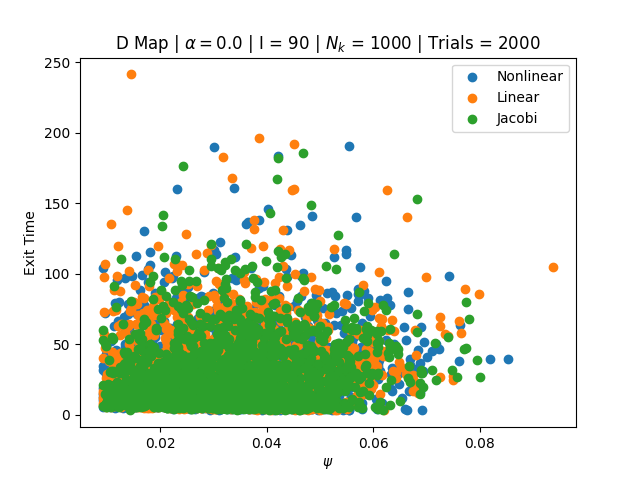
\includegraphics[width=\linewidth]{img/dmap.jpg}
            \caption{$D$ exit subdistribution}
        \end{subfigure}
    
        \begin{subfigure}{0.72\textwidth}
            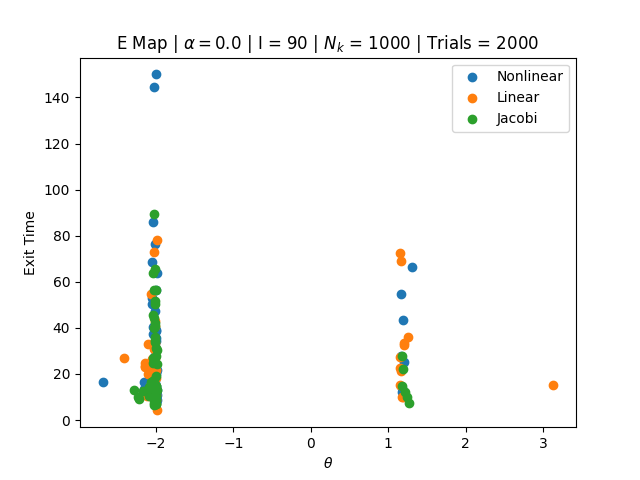
\includegraphics[width=\linewidth]{img/emap.jpg}
            \caption{$E$ exit subdistribution}
        \end{subfigure}
        
        \captionsetup{width=\linewidth}
        \ccaption{$D$ and $E$ exit subdistributions for the IO state. Each trial starts at the point $\theta = 0$ on the curve $C$. Each of the 2000 trials, performed for all three methods, are represented as a dot. Finally, the ``nonlinear'' method in these plots is the CLT model.}
        \label{fig:de-map}

    \end{figure}

    % Discussion of D/E map results
    Qualitatively, the subdistributions in \reffig{fig:de-map} seem to roughly agree with each other. This not only supports the linear approximation, but also confirms the similarity between the Jacobi and CLT models. A more quantitative measure of similarity between these subdistributions has yet to be devised.

    % Code
    The script for checking offending distances for the DO state can be found in \texttt{scripts.docheck}. Variables of interest to change include \texttt{Nk}, \texttt{trials} (the number of trials executed for each $\psi$ and $\psi'$), \texttt{psi\_range} (the values of starting $\psi$ along $L$), and \texttt{psip\_range} (the values of starting $\psi'$ along $L'$). Meanwhile, the \texttt{scripts.contour} script was used to compare the FPE and ULC. A possible variable to change here is \texttt{cdist}, which is simply the radius $r$ of the FPE in $\tilde{\mathbf{x}}$ space, should a different FPE size be desired. Finally, the script \texttt{scripts.elstats} can be used to generate statistics on the FPE, as in \reffig{fig:de-map}. The starting point \texttt{alpha} and trial count \texttt{trials} could be parameters to change here. The reader is encouraged to run the \texttt{scripts.elstats} on different values of $\alpha$ to get more data.

    \pagebreak

    \section{Next Steps}
    T
    % find ez results with lin model

    \pagebreak

    \bibliographystyle{plain}
    \bibliography{bibliography.bib}

\end{flushleft}
\end{document}
